% ===========================================================================
% Energy-Basis Activity Data and the First Measured Number Inside 1A2:
% Electricity Generation Emissions for Pakistan
%
% Target journal: Environmental Modelling & Software (Elsevier)
% Document class: elsarticle, 5p layout
% ===========================================================================

\documentclass[5p,times,authoryear]{elsarticle}

% ===========================================================================
% Shared preamble for every manuscript in this repository.
%
% Papers using it:
%   paper/            agriculture inventory
%   paper_nowcast/    agricultural nowcasting
%   paper_national/   the nine-sector national inventory
%   notes/<sector>/   one data note per non-agriculture sector
%
% It exists because paper/ and paper_nowcast/ began as copies of one another
% and had already drifted five lines apart before a third manuscript existed.
% Eleven copies would drift eleven ways, and a macro that renders differently
% in two papers is the kind of defect nobody notices until proof stage.
%
% \graphicspath is deliberately NOT set here - each manuscript sets its own
% after \input{...preamble}, because figures live beside the document.
% ===========================================================================

\usepackage[utf8]{inputenc}
\usepackage[T1]{fontenc}
\usepackage{amsmath,amssymb}
\usepackage{graphicx}
\usepackage{booktabs}
\usepackage{multirow}
\usepackage{siunitx}
\usepackage[colorlinks=true,citecolor=blue,linkcolor=blue,urlcolor=blue]{hyperref}
% Document-information metadata for every PDF in the bundle (the seventh review noted
% the shipped PDFs carried none). Documents that set their own \hypersetup{pdftitle=...}
% keep it - hyperref takes the LAST setting, and this shared block runs first. Full
% tagged-PDF (tagpdf / \DocumentMetadata) is deliberately not attempted here: the
% installed LaTeX toolchain's support is not uniform across sixteen documents, and a
% half-tagged bundle is worse than an honestly untagged one; deferred deliberately.
\hypersetup{
  pdfauthor={Rehan Ahmad, Pakistan Air Quality Initiative (PAQI)},
  pdfsubject={A reproducible ten-sector national greenhouse-gas inventory
              for Pakistan},
  pdfkeywords={Pakistan, greenhouse gas inventory, IPCC 2006 Guidelines, MRV,
               reproducible research, emissions, air pollutants},
}
\usepackage{caption}
\captionsetup[table]{position=below}
\usepackage{enumitem}
\usepackage{xcolor}
\usepackage{float}
\usepackage{placeins}
\usepackage{tabularx}
\usepackage{natbib}
\usepackage{tikz}
\usetikzlibrary{arrows.meta,positioning,fit,backgrounds}

\setlength{\emergencystretch}{3em}

% Looser float placement to prevent pile-up in two-column mode.
\renewcommand{\topfraction}{0.95}
\renewcommand{\bottomfraction}{0.85}
\renewcommand{\textfraction}{0.05}
\renewcommand{\floatpagefraction}{0.85}
\setcounter{topnumber}{4}
\setcounter{bottomnumber}{3}
\setcounter{totalnumber}{6}

% ---------------------------------------------------------------------------
% Custom shorthand: in macros.tex since the ESSD re-targeting, because the national
% article compiles under the Copernicus class and cannot take this preamble (the class
% loads its own packages) but needs exactly the same macros. This file inputs it so that
% every other manuscript keeps compiling unchanged.
%
% THREE relative paths, because \input resolves against the COMPILE DIRECTORY and not
% against this file, so the depth is a property of whoever is building:
%   ../paper_common      a manuscript compiled from one level down
%   ../../paper_common   papers/<sector>/ and notes/<sector>/
%   ../../../paper_common  paper_national/versions/<v>/, since the national paper was
%                          versioned - that move is what added this third arm, and the
%                          supplement failed with "../../paper_common/macros.tex not
%                          found" until it was here
% A fourth depth needs a fourth arm, which is the cost of keeping a bare `latexmk` in a
% manuscript directory working without a TEXINPUTS set for it.
% ---------------------------------------------------------------------------
\IfFileExists{../paper_common/macros.tex}%
  {\input{../paper_common/macros}}%
  {\IfFileExists{../../paper_common/macros.tex}%
    {% ===========================================================================
% paper_common/macros.tex - the shorthand every manuscript shares.
%
% Split from preamble.tex in the ESSD re-targeting: the national article now compiles
% under the Copernicus class, which loads its own packages and forbids most of what
% preamble.tex sets (geometry-like options, a second hyperref, placeins), but it needs
% exactly the same shorthand as the sector reports. The macros therefore live here, on
% their own, and preamble.tex inputs this file so that every other manuscript keeps
% compiling unchanged. A macro that renders differently in two documents is the defect
% this file exists to prevent; define it once.
%
% Requires: siunitx (for \DeclareSIUnit and \si) - the caller loads it.
% ===========================================================================

% Gas and pollutant names.
\newcommand{\COtwo}{CO\textsubscript{2}}
\newcommand{\COe}{CO\textsubscript{2}e}
\newcommand{\CHfour}{CH\textsubscript{4}}
\newcommand{\NtwoO}{N\textsubscript{2}O}
\newcommand{\NHthree}{NH\textsubscript{3}}
\newcommand{\NOx}{NO\textsubscript{x}}
\newcommand{\SOtwo}{SO\textsubscript{2}}
\newcommand{\PM}{PM\textsubscript{2.5}}
\newcommand{\MCF}{MCF}
\newcommand{\Mt}{\text{Mt~\COe}}
\newcommand{\tCha}{\si{\tonne\per\hectare}}
\newcommand{\AFOLU}{AFOLU}
\newcommand{\GLW}{GLW\,4}
\newcommand{\EFone}{EF\textsubscript{1}}

% siunitx: allow Mt, Tg, ha, head, yr, dB
\DeclareSIUnit{\head}{head}
\DeclareSIUnit{\yr}{yr}
\DeclareSIUnit{\dB}{dB}

% A file name is the one long unbreakable token these documents are full of -
% \texttt{waste\_air\_pollutants\_2024.csv} is wider than a two-column measure and TeX prints
% it past the margin rather than breaking it. Allowing a break AFTER each escaped underscore
% costs nothing and inserts no hyphen, which matters: a hyphenated file name is a wrong file
% name. This is one line because every such name in every document is written with \_.
\let\pkinvunderscore\_
\renewcommand{\_}{\pkinvunderscore\allowbreak}
}%
    {\input{../../../paper_common/macros}}}
% Long unbreakable strings - output filenames, module paths, URLs in \texttt - do not fit a
% two-column measure and TeX prints them past the margin rather than breaking them. Nothing
% read the log, so 47 of those overruns shipped across seven documents. Emergency stretch lets
% the paragraph loosen instead, and \texttt is taught to break at the punctuation these names
% actually contain.
\emergencystretch=6em


% Generated from the current ten-fiscal-year reference release; do not hand edit.
\newcommand{\SectorRefGHG}{45.66}
\newcommand{\SectorRefSOtwo}{30.02}
\newcommand{\SectorLatestGHG}{43.86}
\newcommand{\SectorLatestSOtwo}{5.707}

\graphicspath{{figures/}}

% ---------------------------------------------------------------------------
\journal{Environmental Modelling \& Software}
% ---------------------------------------------------------------------------

\begin{document}

\begin{frontmatter}

\title{PakEmis Sector Technical Note TN02\\[4pt]
A Plant-Resolved, Fuel-Constrained Inventory of Greenhouse-Gas and
Air-Pollutant Emissions from Electricity Generation in Pakistan}

\author[paqi]{Rehan Ahmad\corref{cor1}}
\ead{rehan@pakairquality.com}

\address[paqi]{Pakistan Air Quality Initiative (PAQI), Karachi, Pakistan}

\cortext[cor1]{Corresponding author}

% --- Abstract ---
\begin{abstract}
This technical note documents the power contribution to PakEmis, a shared greenhouse-gas and air-pollutant inventory for Pakistan covering July 2015--June 2025. The reference uncertainty and detailed spatial year remains FY2023--24. Public-power coal is calculated from station consumption and documented rank-specific net calorific values, while generation, heat rates and the publisher's aggregate energy column provide distinct checks and alternatives. Captive gas self-generation is reported under industrial combustion.

The FY2023--24 power calculation module contributes \SI{\SectorRefGHG}{\mega\tonne} \COe{} on AR5 GWP-100, including captive gas; FY2024--25 contributes \SI{\SectorLatestGHG}{\mega\tonne}. Native gas masses and GWP aggregates remain separate. The central air panel admits \SI{\SectorRefSOtwo}{\kilo\tonne} of oil/diesel \SOtwo{} in the reference year and \SI{\SectorLatestSOtwo}{\kilo\tonne} in FY2024--25. Coal and other power pollutants remain separate screening cases because fuel quality and demonstrated control operation are unresolved. Public licence applications establish proposed 92\% and 93\% flue-gas desulfurisation at Port Qasim and China Power Hub, respectively; these design values support explicit selected-plant scenarios, not measured annual stack emissions. Fuel-specific K-Electric coverage alternatives are published separately. The note provides reproducible activity controls, method boundaries and limitations without treating screening endpoints as mathematical bounds.

\end{abstract}

\begin{keyword}
electricity generation \sep captive power \sep energy-basis activity data \sep
coal blend \sep industrial combustion \sep control scenarios \sep
AP-42 \sep IPCC 2006 Guidelines \sep Pakistan \sep MRV
\end{keyword}

\end{frontmatter}

%% Generated by scripts/make_release_cover.py; says which release this documents.
% The Sector Technical Note banner (v1.0.0). Each sector manuscript is a PakEmis Sector
% Technical Note, numbered TN01-TN10 in src/pkinv/release.py (TECHNICAL_NOTES), and says
% so on its first page: it documents ONE sector module of the release named in the block
% that follows, and the national totals are stated only in the data-description article
% (the cover block below reproduces them as release identity, not as a claim of this note).
% Usage, in the document body before the release cover:  \TNBanner{TN01}
\providecommand{\TNBanner}[1]{%
  \noindent\fbox{\parbox{\dimexpr\linewidth-2\fboxsep-2\fboxrule}{%
    \textbf{PakEmis Sector Technical Note #1.} Technical documentation of one sector
    module of the PakEmis release identified below, deposited with the data as part of the
    documentation record. The national data-description article (\texttt{paper\_national/})
    is the only document that states the national totals as its own result.%
    \InputIfFileExists{../../paper_common/generated_availability_tn}{}{}%
  }}\par\medskip}

\TNBanner{TN02}
%% GENERATED by scripts/make_release_cover.py from outputs/release_manifest.json.
%% Do not edit: the edit will be overwritten and CI diffs the result.
\newcommand{\ReleaseCover}{%
\begin{center}\small
\setlength{\fboxsep}{4pt}%
\fbox{\begin{minipage}{\dimexpr\linewidth-2\fboxsep-2\fboxrule\relax}\footnotesize
\textbf{Release provenance.} This document describes PakEmis under the period, configuration and source boundaries specified in its methods. The identifiers below link it to the accompanying products and source register.\\[2pt]
\begin{tabular}{@{}p{0.32\linewidth}@{\hspace{0.03\linewidth}}p{0.65\linewidth}@{}}
Release version & \texttt{1.0.0rc69} \\
Commit & \texttt{d8d874622f9a} \\
Reporting period & July 2015--June 2025 (ten fiscal years) (2015-07-01 to 2025-06-30) \\
Reference & S\_TAN (household survey; TAN nitrogen) \\
FY2023--24 total & 444.61 Mt \COe{} (AR5) under S\_TAN, the reference; 449.85 Mt under L\_TAN \\
Release manifest & \texttt{ac0ffe93ad9fcd88} (SHA-256 of \texttt{outputs/release\_manifest.json}, first 16) \\
Source manifest & \texttt{c1be6d314cfce1ea} (SHA-256 of \texttt{data/manifests/source\_manifest.csv}, first 16) \\
Data-description article & \texttt{paper\_national/} (ESSD, in preparation), same release
\end{tabular}
\end{minipage}}
\end{center}}

\ReleaseCover

% ---------------------------------------------------------------------------
% Main body
% ---------------------------------------------------------------------------

\section{Introduction}
\label{sec:introduction}
Pakistan's thermal fleet combines imported bituminous coal, domestic lignite, gas/RLNG and liquid fuels across CPPA-G/GENCO and K-Electric. NEPRA publishes national fuel controls and plant-level physical fuel, generation and heat-rate records. Their reconciliation provides country-specific activity and boundaries that an aggregate energy table cannot resolve.

This note selects station coal consumption times rank-specific NCV, distinguishes energy from electricity, and tests fuel-specific system coverage. It supports one common GHG and air inventory over July 2015--June 2025. Captive gas is calculated here but reported in industrial combustion. The module's reference-year AR5 total is \SI{\SectorRefGHG}{\mega\tonne} CO$_2$-equivalent; native gases remain separate.

Reviewed oil/diesel SO$_2$ joins the central air panel, while coal/gas/control cases remain separately typed. Public design documents improve selected-plant scenarios without supplying measured annual removal. The contribution is traceable station activity, rank/material accounting and explicit boundary alternatives rather than finer nominal grids alone. Shared national methods and products are documented in the national paper \citep{ahmad2026national}.

% ===========================================================================
\section{Related Work}
\label{sec:related}
% ===========================================================================

\subsection{Fuel-based and generation-based power inventories}

Power-sector emissions can be built from fuel consumed or from electricity generated with an
assumed heat rate. The IPCC 2006 Guidelines describe the fuel route as Tier~1 and treat
generation-based estimates as a fallback where fuel data are unavailable \citep{ipcc2006stationary},
because the heat rate is an efficiency assumption that varies by plant, by load and by year,
and because it is precisely the quantity a compiler is least able to verify.

Pakistan's regulator publishes fuel directly, so the fallback is unnecessary here. This is
worth stating because a workbook consolidating Pakistani plant-level data---which supplied the
captive register used in this paper---computes its \COtwo{} as kilograms per megawatt-hour
derived from IPCC factors through an assumed plant-efficiency range. That is the generation
route, and its output is not used here for that reason, while its plant register is.

\subsection{Coal quality and why the unit matters}

The two coals in Pakistan's fleet are imported bituminous, burned at Sahiwal, Port Qasim and
Hub, and domestic Thar lignite. Published proximate analyses of Thar coal report moisture near
\SI{46}{\percent}, ash around \SI{6.4}{\percent} and calorific values near
\SI{3030}{} kcal/kg---roughly half that of imported steam coal.

That difference is the whole issue. Emission factors expressed per tonne carry it in full;
factors expressed per terajoule do not, because the calorific value is exactly what the
differing energy content describes. The methodological literature on coal inventories treats
blend uncertainty as a major term, and it is---on a mass basis. Section~\ref{sec:methods}
shows it is a \SI{6.8}{\percent} term on an energy basis, which changes what a compiler should
worry about.

\subsection{Captive gas self-generation and the industrial-combustion gap}

Industrial self-generation sits awkwardly in inventory practice. IPCC assigns it to 1A2 with
manufacturing-industry factors, but the data that would support it are usually collected---if
at all---by an electricity regulator whose remit stops at plants selling into the grid.

For Pakistan the consequence is visible in the international comparisons: EDGAR
\citep{edgar2025booklet} reports Pakistani industrial combustion near \SI{44}{\mega\tonne} while most
national compilations report nothing, and the difference between a regulator's scope and an
inventory's scope is a substantial part of that. The activity data that do exist come from a
different regulator entirely---the oil and gas authority, which reports gas delivered to
captive power because it regulates the pipeline rather than the plant.

\subsection{Uncontrolled factors and control-device inventories}

US EPA's AP-42 compilation \citep{epaap42} publishes emission factors for coal, oil and gas
combustion predominantly as \emph{uncontrolled} values, with separate treatment of control
efficiencies, because what leaves a furnace and what leaves a stack differ by up to two orders
of magnitude for particulate and by most of the mass for sulphur.

Applying uncontrolled factors to a fleet with precipitators and desulphurisation, without
saying so, is a well-known way to overstate a power sector's air pollutants by an order of
magnitude. Section~\ref{sec:air} takes the position that where the control inventory does not
exist, the honest output is the uncontrolled bound explicitly labelled as one---not a
plausible-looking estimate resting on an invented removal efficiency.

\section{Scope and activity data}
\label{sec:data}
The common inventory covers ten fiscal years, July 2015--June 2025. NEPRA plant tables provide physical fuel consumption, generation and reported heat rates for named stations. The station ledger distinguishes CPPA-G/GENCO and K-Electric, fuel, coal origin, units and publication table. The latest core year uses the FY2024--25 tables in the State of Industry Report 2025. Later generation-performance editions are independent controls where their periods and system boundaries match.

Coal tonnes consumed are distinct from receipts, inventory change, generation and heat-rate-derived mass. The reference selects physical station consumption and rank-specific NCVs. The published national coal-energy series remains a separate control and structural alternative rather than an additional fuel input. Pre-ledger years retain their documented reconstruction and weaker evidence. Facility commissioning and closure delimit source allocation.

OGRA's annual sector deliveries supply captive gas self-generation: FY2024--25 is 266 MMCFD, the sum of the published SNGPL and SSGC categories. This is gas delivered to industrial self-generation, not all industrial combustion or a complete census of captive fuels. A held administrative plant register supplies geographic support; its fuel sums do not establish annual operation of every listed plant.

Monthly fuel and generation tables provide source-appropriate timing controls. Extraction quality and geographic completeness are tested on the exported records. A twelve-month vector is not national observed activity merely because twelve rows exist. Station-level air admission uses physical oil/diesel mass where available and explicitly identified generation/heat-rate reconstruction for the early years.

% ===========================================================================
\section{Methods}
\label{sec:methods}
% ===========================================================================

\subsection{Grid generation: energy in, energy out}

For each fuel $f$ and gas $g$,
\begin{equation}
E_{g,f} \;=\; A_f \cdot c \cdot EF_{g,f},
\end{equation}
where $A_f$ is the fuel consumed in tonnes of oil equivalent, $c$ the TOE-to-terajoule
constant, and $EF_{g,f}$ the IPCC Table~2.2 default. There is no efficiency term, no heat
rate and no generation figure anywhere in the estimating chain; the plant ledger's generation
data serve only the diagnostics of Section~\ref{sec:validation} and never enter
Equation~(1).

\subsubsection{Why the unit choice is the method}

The coal row hides an unpublished blend. Pakistan burns imported bituminous and domestic Thar
lignite, and NEPRA reports one combined coal figure. IPCC's defaults for the two are:

\begin{table}[htbp]
\centering
\footnotesize
\begin{tabular}{@{}lrrr@{}}
\toprule
\textbf{Coal} & \textbf{kg \COtwo{}/TJ} & \textbf{NCV (TJ/Gg)} & \textbf{kg \COtwo{}/tonne} \\
\midrule
Other bituminous & 94\,600 & 25.8 & $\approx$ 2\,440 \\
Lignite          & 101\,000 & 11.9 & $\approx$ 1\,200 \\
\midrule
\textbf{Ratio}   & \textbf{1.07} & & \textbf{2.03} \\
\bottomrule
\end{tabular}
\caption{The same two coals, two units. Per terajoule they differ by \SI{6.8}{\percent}; per
tonne by a factor of two, because their calorific values differ by \SI{54}{\percent} and
lignite's own published range spans \SIrange{5.50}{21.6}{\tera\joule\per\giga\gram}.}
\label{tab:coals}
\end{table}

An inventory reading tonnes of coal must assume a blend, and that assumption carries most of
the sector's uncertainty. An inventory reading terajoules---which is what tonnes of oil
equivalent already are---carries a \SI{6.8}{\percent} residual instead.

The residual is not assumed away. The sector reports both bounds: all-bituminous gives
\SI{39.00}{\mega\tonne} and all-lignite \SI{40.32}{\mega\tonne}, a span of
\SI{1.32}{\mega\tonne} around a central \SI{40.04}{\mega\tonne} (the grid family's reference; alternatives 38.45 heat-rate, 44.05 with K-Electric, 57.82 legacy control) computed at a
\SI{79}{\percent} lignite share read from the plant fuel ledger
(Section~\ref{sec:factors}).

\subsubsection{No separate oxidation factor}

The 2006 Guidelines assume complete oxidation and fold it into the emission factor;
Table~1.4 carries an explicit oxidation column of \num{1.0} for every fuel. Applying the
1996-vintage \num{0.98} on top would double-discount. This inventory's waste sector
\emph{does} carry an oxidation factor, because open burning genuinely is incomplete, and tests
pin both conventions so neither is "corrected" into the other.

\subsection{Captive gas self-generation: volume to energy to emissions}

OGRA reports a volume and IPCC factors are per terajoule on a net calorific basis, so the
conversion needs a heating value:
\begin{equation}
A \;=\; V \cdot 365 \cdot h \cdot \kappa \cdot \eta,
\end{equation}
where $V$ is MMCFD, $h$ the gross heating value in Btu per standard cubic foot, $\kappa$ the
exact Btu-to-terajoule constant, and $\eta$ the gross-to-net ratio.

Two of those are the assumption. Pakistani pipeline gas runs roughly \SIrange{900}{1000}{}
Btu/scf depending on field and RLNG share, and nothing read here pins it; the utilities bill
in MMBTU at a nominal \SI{1000}{}. Net calorific value is about \SI{10}{\percent} below gross
for natural gas, and omitting that step would overstate the category by \SI{11}{\percent},
because IPCC factors are defined on the net basis.

At \SI{1000}{} Btu/scf the category is \SI{5.55}{\mega\tonne}; at \SI{900}{} it is
\SI{4.99}{\mega\tonne}. Both are reported, as the cement sector reports both clinker ratios.
Everything else in the chain is metered gas or an IPCC default.

\subsection{Two categories, one module}

Grid and captive generation are separate IPCC categories---1A1a and 1A2---computed in one
module, as the transport sector carries road and off-road machinery together. They share the
subject, the plant register and the FY2023--24 reference year; they do not share a
factor table or a
provincial proxy. Nothing downstream conflates them, because the national rollup, the
key-category screen and the completeness table all work on categories rather than modules.

Both categories report FY2023--24: the grid from the 2025 edition's national fuel table,
captive from the same fiscal year's metered gas---one reference year across the sector.

\section{Emission factors and conditional uncertainty}
\label{sec:factors}
Public generation uses the IPCC stationary-combustion energy-industry factors; captive industrial self-generation uses the manufacturing category. The natural-gas factors are 56\,100 kg \COtwo{}, 1 kg \CHfour{} and 0.1 kg \NtwoO{} per TJ in both categories. Coal carbon factors differ by rank. Fuel consumption, rank NCV and factor uncertainties are represented as separate shared parameters, so the same physical fuel draw reaches native gases and applicable air calculations.

The reference coal heat share is the sum of station mass times rank NCV. The historical generation-share series remains a diagnostic and is not an observed fuel-energy share. Rank, moisture/calorific basis and unresolved origin are recorded in the coal account. Alternative fuel-property and coverage cases are not percentiles around the reference.

The tonne-of-oil-equivalent conversion is 0.041868 TJ/t. Its compatibility with the source convention remains relevant for the aggregate non-coal controls. The station-mass coal reference does not inherit the publisher's disputed aggregate coal conversion. For gas, gross heating value and gross-to-net conversion remain explicit conditional assumptions.

Air factors preserve AP-42 source equations and particulate definitions. Sulfur-scaled factors use fuel sulfur once; a controlled factor is not discounted a second time. Unmeasured sulfur specifications and control-operation alternatives are structural cases. The central conditional intervals exclude missing source categories, alternative control configurations and spatial/temporal allocation uncertainty.

\FloatBarrier
% ===========================================================================
\section{Validation}
\label{sec:validation}
% ===========================================================================

\subsection{Pakistan's own UNFCCC filing, cell-audited}
\label{sec:crt}

Pakistan filed Common Reporting Tables with the UNFCCC in 2024, for inventory year 2022. They
are the official statement of what the country reports for this category, and every figure
below is re-derived from the workbook's cells on each run, with the filing's arithmetic
(activity $\times$ implied factor $=$ reported emissions) reproduced exactly before anything
is compared.

The filing reports 1.A.1.a at \SI{777243}{} TJ and \SI{62841}{\kilo\tonne} \COtwo{} for
calendar 2022, and three of its cells matter more than its total.

\textbf{The basis column reads NCV.} Every 1.A.1.a row states the net calorific basis---the
official answer to what Section~\ref{sec:heatrate} approached physically. The sector's largest
declared risk is now covered from two independent directions: the plant meters imply an
efficiency only a net basis supports, and the country's own filing states the basis outright.

\textbf{Gaseous fuels are not estimated.} The official public-electricity category carries NE
for gas, in a country whose regulator reports gas and RLNG as \SI{58}{\percent} of thermal
fuel energy---\SI{306000}{} TJ in this inventory's matched year with no official counterpart.
The filing's liquid-fuel activity is several times the regulator's fuel oil and diesel
combined, so a reallocation may be at work, but as filed the category either omits nearly half
the fleet's fuel or books it unlabelled. This is the kind of finding a cell-level official
comparison exists to surface, and no model comparator could have.

\textbf{The solid-fuel line corroborates two numbers here.} The CRT's \SI{324724}{} TJ agrees
with the regulator's coal energy to \SI{2}{\percent}---two institutions, one answer, which
cuts against the reading of the coal-NCV diagnostic in which the regulator's coal energy is
overstated by most of a factor of two. Section~\ref{sec:impliedcv} now sets a third channel
against both: the per-plant heat rates side with the diagnostic, leaving this agreement as
the counter-evidence rather than the settlement. And its implied \COtwo{} factor of \SI{97.57}{} t/TJ
sits at a \SI{46}{\percent} lignite share on IPCC endpoints: between this paper's superseded
\SI{35}{\percent} and its ledger-derived \SI{79}{\percent}, from 2022 when the Thar fleet was
mid-ramp---consistent with a fleet in transition.

The years overlap by half (calendar 2022 against July 2022--June 2023), so magnitude
comparisons bound rather than test; the fuel-scope and basis findings above do not depend on
the year at all.

\subsection{Grid generation against EDGAR}

EDGAR reports Pakistani power industry emissions at \SI{56.80}{\mega\tonne} \COe{} for 2024
\citep{edgar2025booklet}. This inventory reports the family reference
\SI{40.04}{\mega\tonne} (alternatives 38.45 heat-rate, 44.05 with K-Electric, 57.82 legacy
control) for FY2023--24, or \SI{70}{\percent} of it---different years, so the comparison
bounds rather than tests. That ratio was close to unity on the legacy control and the
direction of the change is not evidence either way:
EDGAR's power figure for Pakistan is built from the same international energy balances that
feed the aggregate fuel control this inventory stopped booking.

EDGAR remains the external benchmark; the official comparison above is the primary one. The taxonomy match is close:
EDGAR's power industry category is essentially 1A1a, built from the same kind of national fuel
statistics, so the comparison is nearly like-for-like rather than approximately so. Agreement
at \SI{142}{\percent} between two independently constructed estimates, in different reference
years, is about as close as this class of comparison gets.

The residual is plausibly captive and industrial self-generation, which NEPRA's scope excludes
and which EDGAR's power category may partly include. That reading is testable now in a way it
was not before: this inventory's captive category is \SI{5.55}{\mega\tonne}, so if EDGAR's
figure included all captive gas generation the two would be further apart, not closer. The
more likely reading is that EDGAR includes some self-generation and this inventory's grid
figure and EDGAR's differ by less than either's uncertainty.

\subsection{Captive gas self-generation against EDGAR's industrial combustion}

EDGAR reports Pakistani industrial combustion at \SI{43.98}{\mega\tonne}. This inventory
reports \SI{5.55}{\mega\tonne} against it, a ratio of \num{0.13}.

That ratio measures \emph{coverage}, not agreement, and the distinction matters enough that
the benchmark row says so explicitly. This category estimates one fuel in one use: gas burned
by industrial plants generating their own electricity. It does not estimate industrial process
heat, boilers, kilns, captive plants burning oil or coal or bagasse, or the kiln fuel behind
the cement category. A ratio near \num{0.13} is therefore the expected result rather than a
discrepancy to investigate, and a ratio near \num{1.0} would indicate an error.

The internal reconciliation is the one that has teeth. The plant register sums to
\SI{288.01}{} MMCFD against OGRA's independently published \SI{288}{}---two sources built from
different records agreeing to \SI{0.01}{}. That is what establishes the category is describing
Pakistan's captive fleet rather than a subset or a superset of it.

\subsection{The time series as an internal check}

\begin{figure}[htbp]
\centering
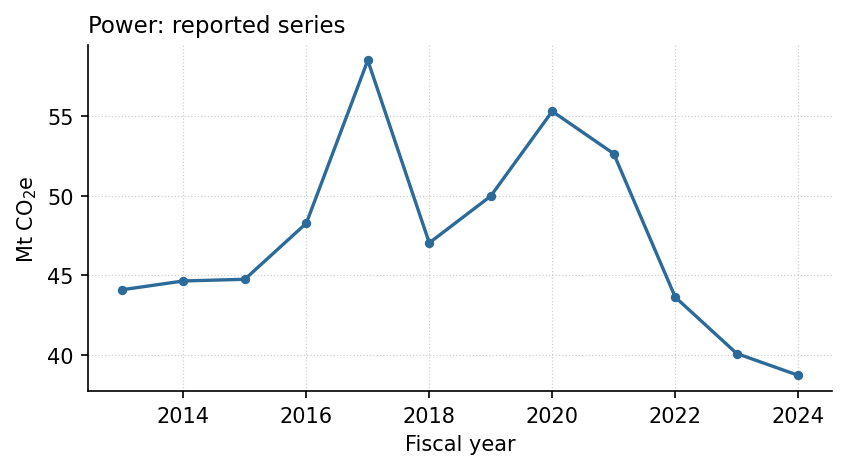
\includegraphics[width=\linewidth]{power_timeseries.png}
\caption{Grid emissions FY2013--24. The furnace-oil era's climb, its one-year collapse in
FY2018--19, the coal-era rise to FY2021--22 and the partial recovery track the fleet's own
history; the added early years parse from five earlier report editions, each reconciled
against its own printed totals.}
\label{fig:series}
\end{figure}

The series now runs eleven years, FY2013--14 to FY2023--24: \SI{44.09}{}, \SI{44.64}{},
\SI{44.75}{}, \SI{48.19}{}, \SI{57.52}{}, \SI{46.84}{}, \SI{49.98}{}, \SI{55.28}{},
\SI{52.51}{}, \SI{43.62}{} and \SI{40.04}{\mega\tonne} (the family reference; alternatives of three kinds: 38.45 heat-rate, a fuel-property alternative; 44.05 with K-Electric, a coverage alternative; 57.82 legacy control, the previously published account)---extended backward in this
revision by parsing five earlier report editions, every added year reconciling against its
edition's own printed Total row, with overlapping years reproduced identically across
editions. The shape is a fleet history: a climb through the furnace-oil era to the
FY2017--18 peak, a \SI{10.7}{\mega\tonne} fall in one year as oil retired, and the coal-era
climb to the FY2021--22 peak. Movements that large correspond to known fleet and demand
events rather than to smooth interpolation, which is what a series built from a modelled
activity proxy would produce.

What those movements were is now decomposed rather than narrated. An additive LMDI-I
decomposition over the fuel table---exact by construction, its terms closing to machine
precision---attributes the \SI{-4.1}{\mega\tonne} change from FY2013--14 to FY2023--24 as
\SI{-5.2}{\mega\tonne} of activity (less fuel energy booked), \SI{0.9}{\mega\tonne} of
mix and \SI{0.2}{\mega\tonne} of factor---and the mix term is close to a pure fuel swap:
coal contributes \SI{+21.0}{\mega\tonne} and furnace oil \SI{-24.2}{}, with gas at
\SI{+4.8}{}. A decade of Pakistani power-sector change is, in megatonnes, one fuel
replacing another.

\textbf{The direction of the total changed with the coal re-base, and the reason is the
activity term.} While the sector booked NEPRA Table 3's coal energy this decade read as a
rise, and this paragraph described the activity term as \emph{more} fuel energy burned.
Booking the generating stations' own metered coal at default rank calorific values instead
lowers the reference year's coal energy by \SI{46}{\percent} and FY2013--14's by only
\SI{36}{\percent}, so the booked total energy falls across the decade where the printed
conversion had it growing. The fuel swap is unaffected---it is a share, not a level---and
the coal and furnace-oil mix terms are what they were. What moved is the level, which was
the part Table 3's flat conversion was setting.
The one year the story is not mix is FY2021--22, whose \SI{-2.8}{\mega\tonne} step was
mostly activity (\SI{-3.2}{}): a demand story rather than a fleet change, in either
direction and on either coal account. The factor term is no
longer zero. An earlier edition applied the FY2023--24 coal blend to every year, so the
term vanished by construction, and this paragraph recorded that as a limitation and
predicted the true series would carry a small positive factor term as the fleet moved from
imported bituminous toward Thar lignite. The per-year blend is wired now---held in
\texttt{data/power\_coal\_blend\_by\_year.csv}, zero before the Thar fleet existed and
\num{0.79} at the reference year---and the prediction held at \SI{+0.2}{\mega\tonne}. The decomposition stays
inside Table~3 deliberately; folding in the generation table would import the coal
coverage mismatch of Section~\ref{sec:heatrate} and narrate an artefact as efficiency.

\subsection{The implied heat rate, and what it says about the activity tables}
\label{sec:heatrate}

The regulator's report contains two tables this inventory had never made talk to each other.
Table~3 gives fuel consumed by fuel; Table~17 gives net generation by fuel and system. Dividing
one by the other gives an implied heat rate---and a heat rate has physical bounds, so the ratio
tests whether the two tables describe the same fleet.

\begin{table}[htbp]
\centering
\footnotesize
\begin{tabular}{@{}lrrl@{}}
\toprule
\textbf{Fuel} & \textbf{Implied efficiency} & \textbf{Spread} & \textbf{Verdict} \\
\midrule
Gas (incl.\ RLNG) & \SIrange{37.7}{56.0}{\percent} & $\times$1.49 & stable \\
Furnace oil       & \SIrange{39.7}{52.1}{\percent} & $\times$1.31 & stable \\
Coal              & \SIrange{34.6}{39.3}{\percent} & $\times$1.14 & unstable \\
Diesel oil        & \SIrange{44.1}{50.2}{\percent} & $\times$1.14 & stable \\
\bottomrule
\end{tabular}
\caption{Implied net efficiency over the nine fiscal years both tables now cover,
FY2015--24, on material years (above \SI{1000}{GWh}).}
\label{tab:heatrate}
\end{table}

Gas is the reassuring row, and the longer window makes it more so, not less. Its implied
efficiency steps from \SIrange{38}{40}{\percent} in FY2015--17 to \SIrange{48}{56}{\percent}
from FY2018 onward---exactly when the RLNG combined-cycle fleet entered service---and then
holds. A ratio of two statistical tables that tracks a known fleet transition and then sits
stably at what combined cycles achieve on a net basis is behaving like real fuel energy
over real generation, in both eras.

Coal is not, on the account this check refuted. Read against NEPRA Table 3's published
coal energy its implied efficiency runs \SI{58.4}{\percent} in FY2020---above any coal plant
ever built, ultra-supercritical included---and \SI{34.6}{\percent} in FY2023--24, a three-fold
swing in four years. No fleet changes efficiency like that. The conclusion is that
Table~3's coal row and Table~17's coal row do not cover the same set of plants, and that the
mismatch moves between years.

Two things follow, and the second matters more than the first.

\textbf{This does not affect the emissions estimate.} The sector is driven by Table~3 alone.
The coverage of Table~17 is irrelevant to Equation~(1), and no number reported in this paper
changes because of the finding. It is published because a reader comparing this inventory's
implied generation against NEPRA's would otherwise discover the discrepancy unaided and have no
way to tell which table this sector used.

\textbf{It partly settles the sector's largest declared risk.} Section~\ref{sec:limitations}
records that the TOE figures may be on a gross rather than net calorific basis, worth
\SIrange{5}{10}{\percent} on \COtwo{}. Gas at a stable \SI{49}{\percent} net is what a combined
cycle does on a \emph{net} basis; read as gross, the same fuel would imply about
\SI{55}{\percent}, which is at the very top of what any fleet average reaches. That is evidence
for the net reading rather than proof of it. The risk stays declared---but it is no longer
untested, which it was for as long as this check went unrun.

The comparison rests on one mapping worth stating. Table~3 has a single ``Gas'' row while
Table~17 splits gas from regasified LNG, and the fuel table has no RLNG row at all---so the
fuel behind Table~17's RLNG generation can only sit inside Table~3's gas figure, there being
nowhere else in the table for it to be. A test asserts that no RLNG fuel row has appeared,
because if a future edition adds one, the mapping would double-count instead.

\subsection{Per-plant heat rates arbitrate the coal conversion}
\label{sec:impliedcv}

The heat-rate instability above asked for the plant-level tables, and the report carries
them: Tables~20, 23 and~28 publish per-plant heat rates in Btu/kWh for five fiscal years,
never previously parsed here. Table~28's footnote states the basis---LHV---so heat rate
times net generation is net-calorific fuel energy, and that energy over the ledger's coal
mass is a calorific value, plant by plant, with Table~3 nowhere in the loop.

Before trusting the channel, the gas plants test it, because for MMBTU-metered plants the
ledger holds true fuel energy. Three behaviours emerge, all reported: three plants (Liberty
Daharki, Sindh Nooriabad-I and -II) print net heat rates that reproduce the ledger's
fuel-over-generation ratio to four digits---fully circular, the heat rate \emph{is} the fuel
table; the pipeline-gas plants Uch and Uch-II sit at \numrange{1.104}{1.109} against the
net-export heat rate, exactly the natural-gas HHV/LHV factor, so same meters converted to
the LHV basis the footnote promises; and the RLNG combined cycles drift year to year, an
independent channel. No coal plant is in the circular set: six of eight print year-varying
operational heat rates, and Sahiwal and Thar Coal Block-I print flat design values (the
latter with a net heat rate below gross, which no plant can do; the cells are kept as
printed and flagged).

The result arbitrates the diagnostic. The Thar mine-mouth plants imply
\SIrange{10.7}{13.9}{} TJ/Gg across their plant-years, mass-weighted \SI{11.1}{} in
FY2023--24---squarely the IPCC lignite value of \SI{11.9}{}---and the imported-coal plants
\SIrange{19.1}{25.1}{}, the bituminous band. The FY2023--24 fleet, mass-weighted at
\SI{99}{\percent} ledger coverage, implies \SI{12.0}{} TJ/Gg against the \SI{24.2}{} that
Table~3's coal energy requires: a factor of \num{2.01}, and \num{1.62} in FY2022--23 at
full coverage. Whether the recovered figures are physical calorific values or the values
NEPRA's own reporting chain assumes is undecidable from this document---and does not matter,
because either reading pins what the official system believes Thar coal's calorific value to
be, and both impeach a conversion that treats the fleet's coal at \SI{24.2}{} TJ/Gg. Two
plant-years fail a sanity screen and are excluded as outliers with their inputs named
(Sahiwal FY2021--22, where the ledger's mass cell is suspect; China Power Hub FY2023--24, a
131.77~kt partial year). As a bonus, Lucky Electric---the ledger's one unresolved coal
origin---implies \SIrange{11.4}{12.1}{} TJ/Gg in all three of its years: lignite-band
evidence that the blend's true value sits near the upper bound of
Section~\ref{sec:factors}'s range.

Two channels now disagree with Table~3's coal row and one agrees with it. The plant heat
rates and the rank-default diagnostic both put the fleet's energy near half the official
figure; the CRT's solid-fuel line agrees with the official figure to \SI{2}{\percent}.
``A scope difference only NEPRA can close'' was this paper's whole statement of the
problem for three releases; the candidate scopes are now enumerated and scored in
\texttt{outputs/power\_table3\_hypotheses.csv}, one row per reading with the held
evidence that bears on it. Of the seven: three are \emph{consistent} with everything
held (an imported-bituminous calorific convention applied to a lignite fleet---the
implied \SI{24.2}{} TJ/Gg sits inside the imported-only band whose mass-weighted value
is \SI{22.99}{}---a gross-basis TOE column, priced at \SI{37.168}{\mega\tonne} and
able to explain only the 0.90 step, and Table~3 being right as published, the CRT's
reading); one is \emph{discriminated against} (K-Electric's ledger fuel is gas and
furnace oil, so its boundary cannot carry a coal factor of two); and three are
\emph{untestable with held sources} (coal stock change, non-power coal inside the
row's scope, and output-derived heat rates---the circularity screen covers
\num{82} plant-fuel comparisons, none of them coal). The register selects nothing:
the estimate keeps Table~3 as its control total under the family's declared
selection rule; the restated case---ledger mass
times per-plant implied calorific value, \SI{190737}{} against \SI{206606}{} TJ---is
published as a labelled sensitivity of \SI{38.45}{\mega\tonne} for the grid category,
the largest labelled case in the totals table. The Energy Yearbook's
conversion-factor note, a paid acquisition this project has not made, would decide
between the leading consistent reading and the CRT's.

\subsection{Climate TRACE, plant by plant}
\label{sec:trace}

Climate TRACE reports \SI{56.19}{\mega\tonne} \COe{} for the Pakistani assets it labels
coal---\SI{2431}{\gram\per\kilo\watt\hour} on its own activity figures, against a
physical ceiling near \SI{1100}{} for coal combustion---where this inventory's coal is
near \SI{21}{\mega\tonne}. That gap has been regression-tested as a total; the per-asset
file, joined to the point-source register, now resolves its structure.

Three findings. First, \emph{every} coal-labelled asset carries exactly
\SI{2431}{\gram\per\kilo\watt\hour}, to the gram---including Fauji Fertilizer's and
Pakistan Steel's captive units, which are not grid plants at all. One modelled intensity
attaches to the label, not to any plant's operation. Second, three pairs of assets report
identical activity and emissions to the megawatt-hour (Balloki/Bhikki/Haveli Bahadur
Shah as triplets; ThalNova with Thar Energy; Lucky with Thar Block~II)---an imputation
signature, sitting exactly where the anomaly is largest. Third, the file carries
misassignments (Hubco typed coal while the ledger records zero fuel burned in FY2023--24;
two Dera Ghazi Khan Cement rows \SI{570}{\kilo\metre} apart) and no year column, so every
comparison bounds rather than tests. Against that: the exact-MMBTU gas plants agree with
the engine at ratios of \num{0.97} to \num{1.03}---the benchmark works where fuels are
metered, and the anomaly is specific to the coal label's factor. That strengthens the
standing reading---upstream Thar mine methane folded into plant rows, or a modelling
artefact---over any reading in which this inventory is missing \SI{36}{\mega\tonne} of
coal combustion.

\subsection{Sentinel-5P sees the fleet}
\label{sec:tropomi}

Every comparator above ultimately rests on statistics someone reported. Sentinel-5P's
TROPOMI instrument \citep{veefkind2012} does not: it measures NO\textsubscript{2} and
\SOtwo{} columns from
orbit, daily, and NO\textsubscript{2}'s hours-scale lifetime keeps the signal near its
source. From a daily \ang{0.1} archive over Pakistan (2020--2026, quality-filtered GEE
\texttt{S5P/OFFL/L3} composites of the Copernicus Level-2 product
\citep{copernicuss5p}; Copernicus Sentinel data, free and open with attribution),
each major generating site's column enhancement over a same-day
\SIrange{0.3}{0.7}{\degree} annulus background was extracted for 2,275 days---nine
sources, with complexes the grid cannot separate treated as one source each and labelled
so---then aggregated to season-balanced fiscal years (300+ valid days behind most annual
means). Four hypotheses were stated before the full run, each keyed to something the
ledger already claims.

\textbf{The Thar ramp is decisively visible.} As the mine-mouth cluster went from one
plant to four and \SI{3.6}{} to \SI{13.2}{\mega\tonne} of coal, its NO\textsubscript{2}
enhancement rose \num{2.2}-fold (FY2019--20 to FY2023--24) and its \SOtwo{}
enhancement---the lignite sulfur signature---\num{9.0}-fold, from \SI{9.6e-6}{} to
\SI{8.6e-5}{\mole\per\metre\squared}: the strongest signal in the study, and an
independent witness to the build-out the LMDI decomposition quantifies from the fuel
side.

\textbf{The Hub site fades exactly as the ledger retires it.} Hubco's furnace oil fell
\SI{977}{\kilo\tonne} to zero and China Power Hub's imported coal \SI{2253}{} to
\SI{132}{\kilo\tonne}; the site's enhancement halves, FY2020--21 \SI{1.8e-5}{} to
FY2023--24 \SI{9.3e-6}{\mole\per\metre\squared} (ratio \num{0.53} against a pre-stated
threshold of 0.65). The FY2024--25 rebound in the satellite series sits beyond the
ledger's coverage and is reported as an observation, not a verdict.

\textbf{The satellite arbitrates the Sahiwal FY2021--22 mass cell.} The heat-rate
channel flagged that year's ledger coal mass as suspect (\SI{1444}{\kilo\tonne} against
\SI{6881}{GWh}, implied CV \SI{44}{} TJ/Gg). Generation says the year ran at \num{0.94}
of the previous one; the suspect mass says \num{0.53}. The satellite---which cannot read
NEPRA's tables---says \num{1.02}, siding with generation and independently corroborating
a data-quality flag raised by an entirely different method. The following year, when
generation genuinely collapsed, the enhancement fell to \SI{1.3e-6}{}: the instrument
tracks the plant.

\textbf{Rank agreement, and an honest control.} Pooling within-source ranks across 36
source-years, fiscal-year enhancement orders the years the way ledger generation does:
Spearman $\rho = 0.58$, $p = 2\times10^{-4}$ (the Thar cluster alone: $\rho = 1.0$). Uch,
the steady field-gas null control, holds flat (CV \num{0.17}). Guddu was drafted as a
second null and the data rejected the premise---its fuel really does swing by a third
across the window, and its enhancement follows---which is covariation evidence, honestly
reclassified rather than a failed control.

The limits are declared with the channel. No wind rotation: plume smearing into the
annulus biases every enhancement \emph{low}, making the detections conservative. The
Port Qasim complex sits inside Karachi's plume and supports only within-source time
contrasts. The columns are daily L3 composites without averaging-kernel handling, and
nothing here converts a column to a mass emission rate---this channel ranks and tracks;
it does not weigh. Nothing in it feeds the estimate.

\subsection{The K-Electric leg, made decision-ready}
\label{sec:keleg}

The boundary audit finds, in every year, that the plant sum brackets the national gas row
only when the K-Electric system is excluded---which favours the reading that Table~3 omits
K-Electric and is not proof of it. The furnace-oil rows point the other way in four of the
five years, the sum with K-Electric sitting closer to the national row than the sum
without it. The FY2023--24 furnace-oil year is the exception and the sharpest discriminator
in the panel: the without-K-E plant sum sits at \num{0.890} times the national RFO row and
the with-K-E sum at \num{1.256} times it, because K-Electric's furnace oil collapsed in the
same year the national row did. Whether the national fuel statistic already contains
K-Electric's fuel is therefore not established.

The whole ladder now ships as one table
(\texttt{outputs/power\_toe\_reconciliation.csv}, rc30): per year and fuel, the national
Table-3 energy (recovered from the audit's own ratio pair, so the table carries no
calorific constant of its own), the CPPA plant sum, the K-Electric plant sum and the
heat-rate-implied coal energy, side by side. It settles nothing the configurations leave
open---settling needs HDIP's conversion-and-scope metadata, the one paid or written-answer
item in this sector---but it puts every rung of the comparison in one place. When that
metadata arrives, the family's names map onto the resolution the eighteenth review
proposed: \texttt{inventory\_reference} is the \emph{hdip-toe-reported} reading,
\texttt{power\_plant\_physical\_coal} the \emph{plant-physical-NCV} reading, and
\texttt{power\_with\_kelectric} the \emph{hdip-toe-plus-KE} reading.

What that boundary question is worth is now computed rather than gestured at, and it is
not the flat five-to-six megatonnes earlier versions of this paper carried. The K-E ledger
rows imply \SI{7.1}{}, \SI{7.7}{}, \SI{6.3}{}, \SI{4.9}{} and \SI{4.0}{\mega\tonne}
\COtwo{} across FY2019--24: a \SI{48}{\percent} decline in five years, driven almost
entirely by furnace-oil retirement (\SI{977}{} down to \SI{209}{\kilo\tonne}) while gas
collapsed into RLNG. Whichever way the boundary decision goes, the correction is a trend,
not an adder; the coverage alternative is priced for all nine panel years in
\texttt{outputs/pakemis\_structural\_trajectories.csv} (axis \emph{power scope}). Two
corroborations ride along: implied net efficiency rises from
\SI{36.9}{} to \SI{45.5}{\percent} across the window---what RFO steam giving way to RLNG
combined cycle should do, and a check that the volume-based heating-value assumption is
not badly wrong---and the arithmetic reproduces the boundary audit's energies exactly.

The case is published as the coverage alternative ``grid + K-Electric ledger fuel'':
\SI{44.05}{\mega\tonne} against the \SI{40.04}{} headline, priced beside the reference and
not added to it, because adding it would count K-Electric's fuel twice if the national
statistic already contains it. Its evidence classes are
weaker than the CPPA leg's---volumes at an assumed heating value, oil at default
calorific values, only the two Nooriabad units metered exactly---and that weakness, with
the open boundary question, is what keeps it an alternative rather than a category.

\subsection{What is not validated}

Fuel quality. Nothing here tests the coal blend, the calorific values, the TOE convention or
the gas heating value against a Pakistani laboratory measurement, because none is published
in anything read here. Those four questions carry this sector's real uncertainty, and the
uncertainty statement now says so in kind rather than in width: the blend and the heating
value are parametric with ranges read off their corroborations, while the calorific and
conversion questions are one-sided structural cases in Table~\ref{tab:scenarios}, each with
a conditional interval and no probability---because a $\pm$ percentage that absorbed a
factor-of-two question would misdescribe both the question and the percentage.

\paragraph{Which basis the historical years should use.}
NEPRA's per-plant generation panel covers FY2015--16 to FY2019--20 and the plant fuel ledger
begins in FY2019--20, so exactly one fiscal year carries both, and that year decides which
provincial vector the earlier years should take. Emissions follow fuel rather than generation,
so the fuel vector is the control and the two candidates are the panel's own-year generation
and the reference-year vector the release would otherwise borrow for every period. The
comparison ships per stream and province as
\texttt{outputs/pakemis\_power\_grid\_basis\_change.csv}. Measured as total-variation
distance from that control, furnace oil's own-year generation lands at \num{0.005} against
\num{0.066} for the borrowed vector; for gas the ordering reverses, and the borrowed vector is
much the closer of the two. Generation shares equal fuel shares only where plants burn at a
common heat rate: the furnace-oil fleet is near enough uniform for that to hold, and the gas
fleet---Punjab's RLNG combined cycle against the low-BTU plants in Balochistan---is not.
On that comparison furnace oil was allocated on own-year generation for the five years the
panel reaches and gas was left on the reference vector, through release 1.0.0rc65. Neither is
applied now. The comparison had been run on a panel holding under half of that year's gas
generation, and the question it posed was the wrong one: the same report tables print each
station's fuel quantity beside its generation, so the earlier years take the fuel itself.
From rc66 every fuel is split between provinces by each year's own station fuel record
(\texttt{outputs/pakemis\_power\_provincial\_basis\_by\_year.csv}), coal by station tonnage
at the calorific value the national account books it at; the comparison above remains as the
record of how far generation sits from fuel.

% ===========================================================================
\section{Results}
\label{sec:results}
% ===========================================================================

\subsection{The sector}

\begin{table}[htbp]
\centering
\footnotesize
\begin{tabular}{@{}llrr@{}}
\toprule
\textbf{Category} & \textbf{IPCC} & \textbf{Mt \COe{}} & \textbf{$\pm$\%} \\
\midrule
Electricity and heat production & 1A1a & 40.040 & 10.9 \\
Captive gas self-generation     & 1A2  &  5.549 & 15.2 \\
\midrule
\textbf{Total}                  &      & \textbf{45.590} & \textbf{9.7} \\
\bottomrule
\end{tabular}
\caption{Electricity generation, both categories on FY2023--24. The uncertainty column is
Approach~1 per category and for the sector, with the four grid fuel rows' activity errors
treated as fully correlated through the shared TOE conversion (independently they would
give \SI{7.3}{\percent}); the one-sided questions---the coal conversion, the TOE basis,
K-Electric coverage---are structural cases in Table~\ref{tab:scenarios}, not width in
this column.}
\label{tab:results}
\end{table}

\begin{figure}[htbp]
\centering
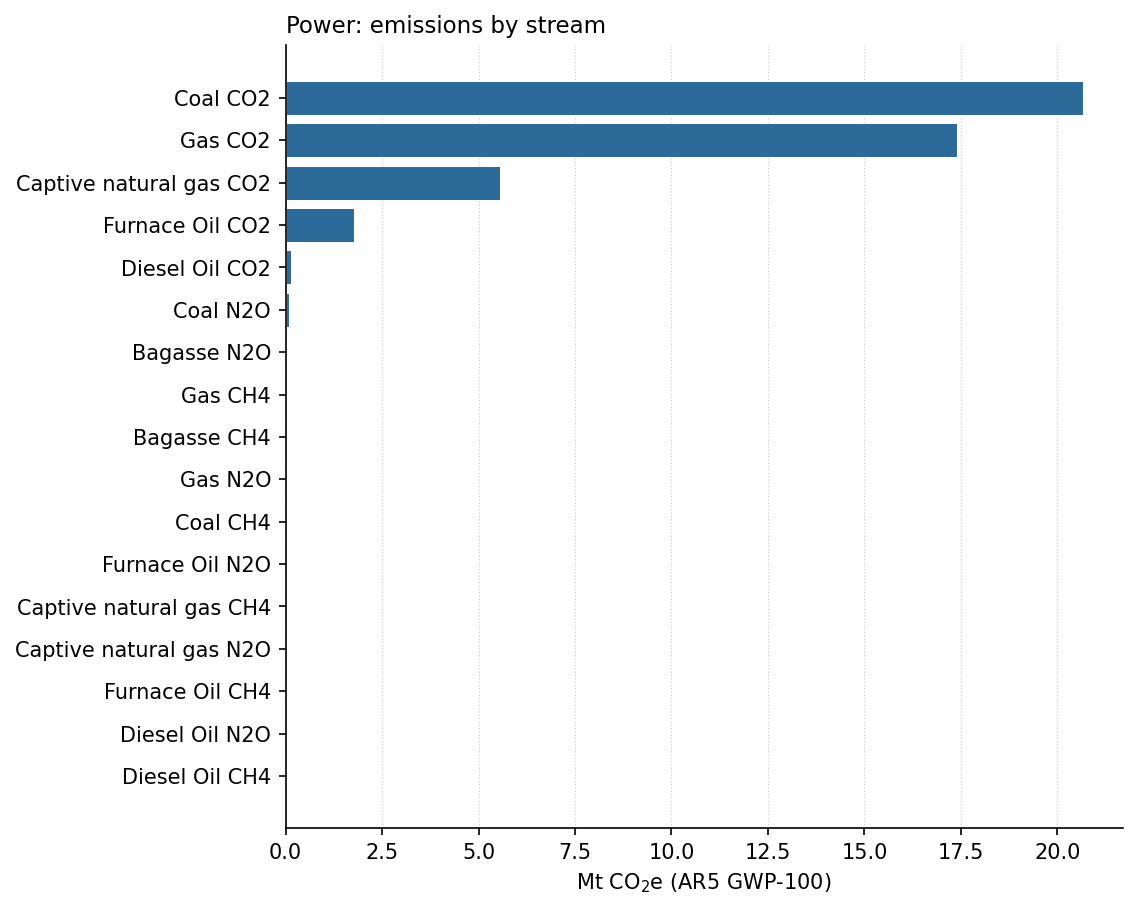
\includegraphics[width=\linewidth]{power_streams.png}
\caption{Emissions by fuel and gas. The sector is \SI{99.6}{\percent} \COtwo{}: the utility
\CHfour{} and \NtwoO{} factors in Table~2.2 are small precisely because large boilers burn
completely.}
\label{fig:streams}
\end{figure}

Coal is \SI{20.59}{\mega\tonne} of \COtwo{}, gas \SI{17.40}{\mega\tonne}, furnace oil
\SI{1.79}{\mega\tonne} and diesel \SI{0.13}{\mega\tonne}. Coal is \SI{37.9}{\percent} of the
energy and \SI{51}{\percent} of the grid emissions, which is the carbon-intensity difference
between coal and gas expressing itself directly---and the reason a fleet shifting between them
moves emissions faster than it moves generation.

The grid category now carries the sector's smallest stream and its first memo item. Eight
sugar-mill cogeneration plants sold \SI{726.85}{GWh} of bagasse-fired electricity to the
grid in FY2023--24 (Table~8's E3 block, reconciled against its printed total); at IPCC
biomass factors that is \SI{0.02}{\mega\tonne} of \CHfour{} and \NtwoO{}---the one
non-fossil methane in the sector, at AR5~28---and \SI{1.09}{\mega\tonne} of biogenic
\COtwo{} reported as a memo outside every total, the carbon having been fixed by the same
season's cane. The activity is generation times an assumed \SI{15000}{\kilo\joule\per\kilo\watt\hour}
heat rate, the sector's one generation-derived stream, and it is labelled structurally
weaker than the metered-fuel streams for exactly that reason. Three plants list biomass and
one lists furnace oil as its alternate fuel; no source read here publishes the co-firing
share, so the furnace-oil caveat is named rather than split.

\subsection{Sensitivities}

\begin{table}[htbp]
\centering
\footnotesize
\setlength{\tabcolsep}{4pt}
\begin{tabular}{@{}p{0.32\linewidth}rp{0.36\linewidth}@{}}
\toprule
\textbf{Case} & \textbf{Mt \COe{}} & \textbf{What it bounds} \\
\midrule
All coal bituminous & 38.995 & lower bound, grid \\
Reported (79\% lignite) & 40.040 & \\
All coal lignite    & 40.318 & upper bound, grid \\
Coal at implied CVs & 38.452 & the conversion question, grid (Sec.~\ref{sec:impliedcv}) \\
Table 3 published energy & 57.820 & legacy published control, grid \\
\midrule
Captive at 900 Btu/scf & 4.995 & lower bound, 1A2 \\
Reported (1000 Btu/scf) & 5.549 & \\
\bottomrule
\end{tabular}
\caption{Both published assumptions, bounded. The coal blend spans \SI{1.32}{\mega\tonne} on
the family reference \SI{40.04}{} (alternatives 38.45 heat-rate, 44.05 with K-Electric,
57.82 legacy control); the gas heating value spans \SI{0.55}{\mega\tonne} on \SI{5.55}{}.
The last row is the aggregate fuel control booked before the coal re-base, kept here so the
blend span and the account change are not read as one quantity.}
\label{tab:sensitivity}
\end{table}

\begin{figure}[htbp]
\centering
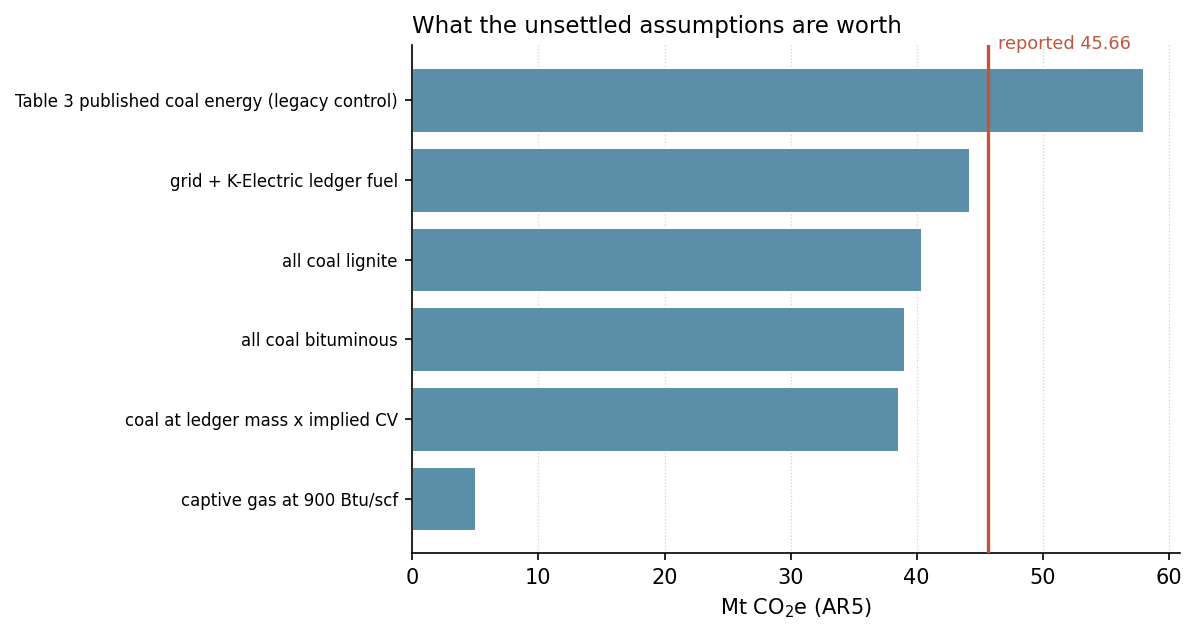
\includegraphics[width=\linewidth]{power_sensitivity.png}
\caption{The same as a range around the reported figure.}
\label{fig:sensitivity}
\end{figure}

Neither span is large relative to the sector, and that is the result. On a mass basis the coal
row alone would span roughly a factor of two; on an energy basis it spans
\SI{3.3}{\percent} of the grid category. The account change is a separate and larger matter
and is kept separate: the legacy control sits \SI{17.78}{\mega\tonne} above the reference,
which is \num{13} times the blend span, and no reading of the blend reaches it.

\begin{table}[htbp]
\centering
\footnotesize
\begin{tabular}{@{}lrrr@{}}
\toprule
\textbf{Structural case} & \textbf{Mt \COe{}} & \textbf{P2.5} & \textbf{P97.5} \\
\midrule
Reference (family reference)  & 40.040 & 36.0 & 44.5 \\
All coal bituminous           & 38.995 & 34.9 & 43.4 \\
All coal lignite              & 40.318 & 36.1 & 44.9 \\
Coal at implied CVs           & 38.452 & 34.4 & 42.9 \\
Table 3 published energy      & 57.820 & 51.8 & 64.3 \\
TOE on a gross basis          & 37.168 & 33.3 & 41.4 \\
Grid + K-Electric ledger fuel & 44.054 & 39.8 & 48.5 \\
\midrule
Captive at 900 Btu/scf        &  4.995 &  4.3 &  5.8 \\
\bottomrule
\end{tabular}
\caption{The one-sided questions as named cases, each with a conditional parametric
interval and no structural probability. Discrete choices are kept unsampled so a
confidence interval cannot conceal a boundary or coverage choice; the parametric
$\pm$\SI{10.9}{\percent} above is conditional on the reference configuration of every row
in this table.}
\label{tab:scenarios}
\end{table}

\subsection{Provincial allocation, corrected}

\begin{figure}[htbp]
\centering
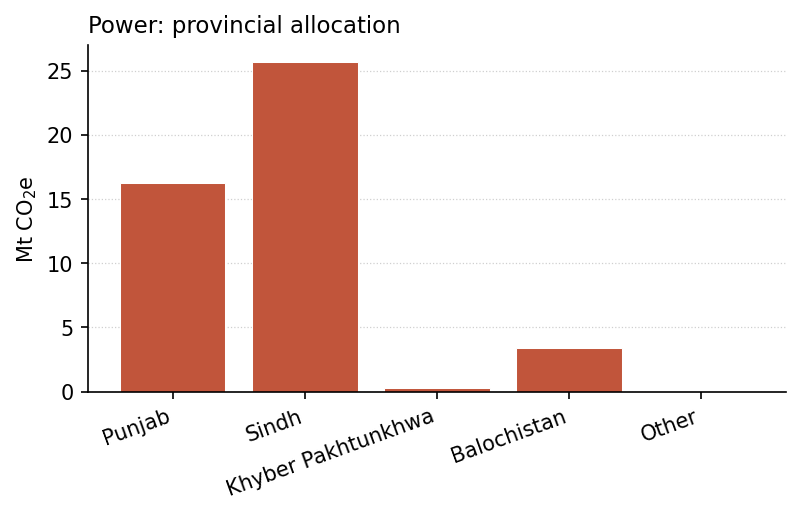
\includegraphics[width=\linewidth]{power_provincial.png}
\caption{Punjab \SI{16.24}{\mega\tonne}, Sindh \SI{25.67}{\mega\tonne}, Balochistan
\SI{3.41}{\mega\tonne}, Khyber Pakhtunkhwa \SI{0.27}{\mega\tonne}. Unlike almost every other
sector in this inventory, the ordering does not follow population, because it follows the
plants---and above all the Thar coalfield.}
\label{fig:provincial}
\end{figure}

This geography has now been corrected twice, each time by a better class of evidence, and
the second correction is larger than the first. The original capacity proxy gave Khyber
Pakhtunkhwa \SI{14.24}{\percent} of a combustion sector whose electricity there is hydro;
plant-wise generation moved \SI{6.2}{\mega\tonne} out of that province. But the generation
proxy still blended all fuels onto one share, and the ledger joined to the report's own
plant-location table (Table~5) shows the fuels do not share a geography: coal is
\SI{89}{\percent} Sindh on the stations' booked energy (four Thar mine-mouth plants, Port Qasim and
Lucky against Sahiwal alone in Punjab), the RLNG combined-cycle corridor is Punjab, the
pipeline-gas plants sit on the Sindh and Balochistan fields, and the furnace oil actually
burned in FY2023--24 is entirely Punjab---Hub, the Balochistan plant that dominated older
vintages of this split, reports zero fuel for the year. Allocating each fuel on its own
plants moves \SI{12.6}{\mega\tonne} from Punjab to Sindh at an unchanged national total
and makes Sindh, not Punjab, the sector's dominant province. Each per-fuel share is
recomputed from the ledger by a test, so the committed geography cannot quietly outlive
its derivation; the energy weights carry their evidence classes (MMBTU exact, volumes at
the declared heating value, coal mass at the per-plant implied calorific values of
Section~\ref{sec:impliedcv}). \ref{app:provincial} records the replaced proxies.

\subsection{Contribution to the national inventory}

\begin{table}[htbp]
\centering
\footnotesize
\begin{tabular}{@{}lrr@{}}
\toprule
\textbf{Category} & \textbf{Level (\%)} & \textbf{Variance (\%)} \\
\midrule
Electricity and heat production & 9.00 & 0.80 \\
Captive gas self-generation (1A2)        &  1.25 & 0.03 \\
\bottomrule
\end{tabular}
\caption{Shares of the national total and of national Approach-1 variance.}
\label{tab:keycat}
\end{table}

Grid generation is the third largest category in Pakistan and---since the uncertainty
rebuild---no longer a large contributor to national variance: \SI{0.80}{\percent}, down
from a published \SI{3.24}{}, and from an earlier vintage in which it ranked second after
enteric fermentation. The fall is not new information about the fleet; it is the flat
activity percentage being replaced by per-fuel widths the evidence supports, and the
questions actually worth megatonnes---the coal conversion, the TOE basis, K-Electric
coverage---moving to the structural-scenario table where a probability interval cannot
conceal them. The honest summary is that this sector's parametric uncertainty is modest
and its structural uncertainty is large, one-sided and named.

Captive gas self-generation contributes \SI{0.03}{\percent} of national variance, which is the expected
result for a category whose activity is metered and whose factor is an IPCC default: its
\SI{15.2}{\percent} band is small and its size is modest. Its value to the inventory is not
uncertainty reduction but coverage---it is the first number inside a gap that was previously
empty.

\FloatBarrier
% ===========================================================================
\section{Air Pollutants: An Upper Bound, and a Re-Diagnosed Blocker}
\label{sec:air}
% ===========================================================================

\subsection{The blocker was fuel analysis, not emission factors}

This sector's air-pollutant layer was previously recorded in this inventory's completeness
table as not estimated, blocked on EMEP/EEA large-combustion factors that the agency no longer
serves in a retrievable form. Working back to the primary tables showed that diagnosis was
wrong, and correcting it is a more useful result than the layer itself.

US EPA's AP-42 gives no coal \SOtwo{} factor as a fixed value. For bituminous coal,
Table~1.1-3 publishes $38S$, where $S$ is the sulfur weight percent of the coal actually
burned; for lignite---which is what \SI{79}{\percent} of this fleet's coal energy is---the
separately fetched Section~1.7 publishes $30S$ (its own footnote scales the factor $22S$ to
$34S$ with ash sodium, which is not held here, so the table's default is carried).
Table~1.3-1 publishes $157S$ for No.~6 fuel oil. Filterable particulate is $10A$
(bituminous, Table~1.1-4) and $6.5A$ (lignite, Table~1.7-4), functions of ash content.

The factors were never missing. What is missing is the \emph{fuel analysis} they scale with,
and NEPRA publishes none. That is a different problem with a different solution: no amount of
searching for factor tables would have closed it, and the earlier note would have sent a
reader looking in the wrong place.

\subsection{Fuel quality as a published range}

Published Thar lignite sulfur spans \SIrange{0.26}{2.90}{\percent}---a factor of eleven.
Ash is better constrained, with two published means at
\SI{6.42}{} and \SI{6.83}{\percent}.

Sulfur and ash are therefore carried as ranges, with the central value the geometric mean and
the uncertainty read off the range---the same treatment this inventory's fugitives sector gives
IPCC's published factor ranges, using the same function so the two cannot drift apart on the
convention. The Thar ranges belong to the lignite share by construction; the imported
bituminous burned at Sahiwal, Port Qasim and Hub has no consignment analysis in anything read
here, so the bituminous share carries the same ranges as a \emph{declared proxy}---imported
bituminous is typically lower-sulfur than this range's centre, so if anything the bituminous
side of the bound is generous, and the proxy is recorded in the fuel-quality file rather than
silently reused.

\subsection{The coal rank split, and why it raised the bound by half}

Coal was previously one stream on the bituminous section. Since the Thar-lignite split,
\SI{79}{\percent} of the coal energy (\texttt{coal\_lignite\_share}, generation-weighted
from the plant fuel ledger, $\pm$\SI{12}{\percent}) rides Section~1.7's own factors and
lignite's IPCC net calorific value of \SI{11.9}{\tera\joule\per\giga\gram}, the remainder
Section~1.1's on \SI{25.8}{}. The rank split moves the bound substantially \emph{upward}:
a tonne of lignite carries less than half the energy of a tonne of bituminous coal, so a
per-tonne factor scaled by the same sulfur or ash nearly doubles per terajoule---the same
arithmetic through which the greenhouse-gas layer's rank blend works, now applied where it
bites hardest. The firing configuration is a declared assumption (pulverized dry-bottom
tangential, the configuration whose \NOx{} factor Section~1.7 rates A); no Pakistani
document read here states the Thar boilers' firing arrangement. Lignite CO is ND in
Table~1.7-1 for this configuration and is therefore absent rather than zero-filled. Grid
bagasse cogeneration enters the layer from Section~1.8 on the same fuel energy the
greenhouse-gas layer burns---uncontrolled filterable PM and \NOx{} only, because the
section publishes no \SOtwo{} or CO factor for bagasse, whose sulfur it describes as
characteristically negligible.

\subsection{The result, labelled as what it is}

\begin{table}[htbp]
\centering
\footnotesize
\begin{tabular}{@{}lrl@{}}
\toprule
\textbf{Pollutant} & \textbf{kt/yr} & \textbf{AP-42 source} \\
\midrule
PM (filterable) & 362.3 & 1.7-4 ($6.5A$), 1.1-4 ($10A$), 1.8-1, 1.4-2 \\
\SOtwo{}        & 208.7 & 1.7-1 ($30S$), 1.1-3 ($38S$), 1.3-1 ($157S$), 1.4-2 \\
\NOx{}          & 113.4 & 1.7-1, 1.1-3, 1.3-1, 1.8-1, 1.4-1/3.1-1 \\
PM\textsubscript{10} & 118.3 & 1.7-7 ($2.3A$), 1.1-4 ($2.3A$), 1.4-2 \\
PM\textsubscript{2.5} & 34.3 & 1.7-7 ($0.66A$), 1.1-6 ($0.6A$), 1.4-2 \\
CO              &  11.9 & 1.1-3, 1.3-1, 1.4-1 \\
VOC             &   0.7 & 1.4-2 \\
\bottomrule
\end{tabular}
\caption{Grid only, FY2023--24 fuel, \textbf{uncontrolled}---an uncontrolled
screening scenario, each coal rank on its own AP-42 section since the Thar-lignite split.
Captive self-generation is IPCC 1.A.2 and is priced once, in the industrial air layer
(engine and turbine factors), so it no longer appears here.
Applied to the same terajoules
the greenhouse-gas layer burns, so both inventories describe the same combustion.}
\label{tab:air}
\end{table}

\begin{figure}[htbp]
\centering
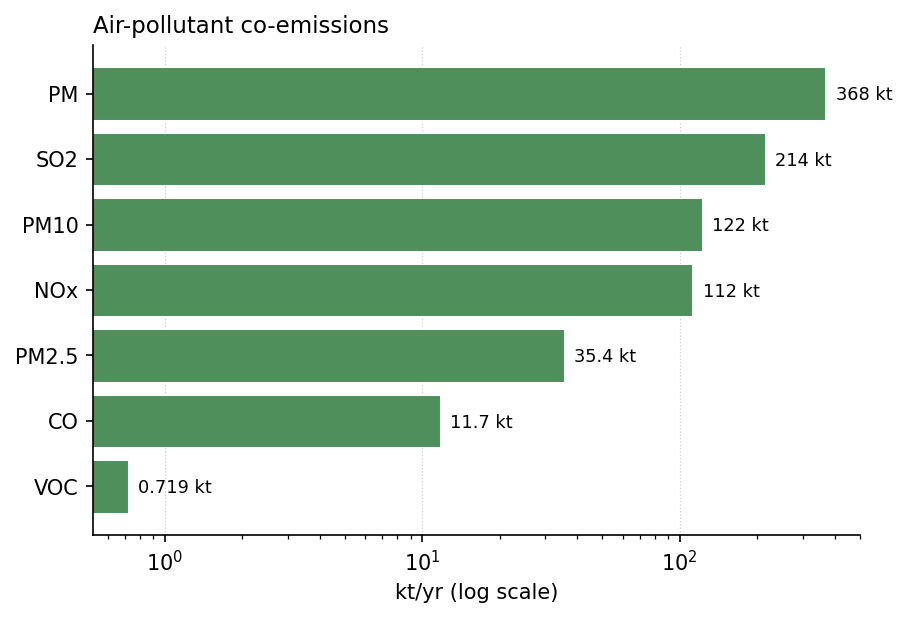
\includegraphics[width=\linewidth]{power_air.png}
\caption{The same figures on a log axis, which the range demands.}
\label{fig:air}
\end{figure}

\textbf{These are uncontrolled factors, and that word carries the whole caveat.} AP-42's
uncontrolled rows describe what leaves the furnace, not what leaves the stack. Pakistan's
supercritical coal units were built with electrostatic precipitators and the newer ones with
flue-gas desulphurisation, which remove most of the particulate and much of the sulphur. No
national dataset records which control is fitted where or how it performs.

Applying a removal efficiency would therefore mean inventing the number that matters most---it
spans an order of magnitude between uncontrolled and well-controlled. The bound is reported as
a bound, and the estimate of what the fleet actually emits is left not estimated, with the
missing parameter named. A number labelled as a bound is useful; the same number labelled as
an estimate would not be.

Where that parameter lives is now established rather than guessed. All five of NEPRA's
Licensees HSE Performance Evaluation Reports (2021 through 2024--25) were obtained and
audited for this revision: they publish no per-plant control equipment, emissions or
measurements---they are occupational-safety scorecards, one aggregate points total per
company---but their evaluation questionnaire scores licensees on ``pollution control
measures related to air quality'' and on whether an environmental monitoring report was
submitted. The controlled-emissions data this layer needs therefore exists at the
regulator as unpublished licensee submissions under the Power Safety Code, and the
concrete route to it is a request to NEPRA's HSE department, not a further search of the
published record.

\subsection{PM\texorpdfstring{\textsubscript{2.5}}{2.5} from the size distribution, with its
own check}

An earlier version of this layer carried no PM\textsubscript{2.5} row, deliberately: AP-42
Table~1.1-4 gives filterable PM and PM\textsubscript{10} for coal but no
PM\textsubscript{2.5}, and reporting the gas figure alone---about \SI{1}{\kilo\tonne},
because AP-42 notes all gas particulate is under a micron---would have read as power being
negligible for fine particulate against residential biomass at \SI{282}{\kilo\tonne} under
that sector's reference configuration, which
uncontrolled coal is not.

The missing piece was the cumulative particle-size distributions---and each rank has its
own. Table~1.1-6 (bituminous, dry-bottom pulverised) puts \SI{6}{\percent} of filterable
mass at or below \SI{2.5}{\micro\metre}: a cumulative factor of $0.6A$~lb/ton, which the
table rates C---below the A of the mass factor it scales, as a derived number should be.
The same distribution puts \SI{23}{\percent} at or below \SI{10}{\micro\metre}, $2.3A$,
exactly the PM\textsubscript{10} factor Table~1.1-4 already supplied; the two tables
reproducing each other is the check on the transcription. Lignite's own Table~1.7-7 is
coarser-shifted but sits on a heavier per-terajoule mass: \SI{10}{\percent} at
\SI{2.5}{\micro\metre} ($0.66A$) and \SI{35}{\percent} at \SI{10}{\micro\metre} ($2.3A$) of
the $6.5A$ tangential filterable factor. The result is \SI{34.32}{\kilo\tonne} of
uncontrolled PM\textsubscript{2.5}, \SI{33.31}{} of it from coal---roughly double the
pre-split figure, because lignite's tonnage per terajoule doubles the ash-scaled
mass---carried with the same
bound-not-estimate caveat as every row above---and for fine particulate that caveat bites
hardest, because electrostatic precipitators remove fine mass least efficiently exactly
where the health burden concentrates.

\subsection{A convergence that dissolved, which is the more instructive record}

The consolidated plant workbook that supplied this paper's captive register computes its own
grid \SOtwo{} for 2024, on a generation basis with kilogram-per-megawatt-hour factors, at
\SI{253.2}{\kilo\tonne}. Before the rank split, the AP-42 fuel-basis figure sat within
within a few per cent of it, and an earlier edition of this section recorded that agreement
with the warning that it was a coincidence of assumptions rather than corroboration---both
routes embedded the same all-bituminous reading of the coal fleet. The rank split proved
the warning right by dissolving the agreement: on each rank's own section and calorific
value the figure is \SI{208.7}{\kilo\tonne}, \SI{17.6}{\percent} below the workbook---it
read \SI{399.4}{\kilo\tonne} until rc60, when the oil and diesel share of this screening
narrowed to the fuel the plant-level admission register does not price, and higher again
until the coal re-base, which moved it to the other side of the workbook. That reversal is the same point made twice: this screening is coal energy times
a sulphur content, so it tracks whichever coal account is booked, while the workbook's
\SI{253.2}{\kilo\tonne} does not move at all. The agreement was never evidence and
neither is the disagreement's direction. The
divergence now \emph{measures} the shared assumption the old agreement concealed. Two
estimates that guessed the same missing parameter agreed; correcting the parameter on one
side moved it, which is exactly what agreement-by-shared-guess predicts and
corroboration does not.

\subsection{Gas \texorpdfstring{\NOx{}}{NOx}: the ledger settles the combustor question,
with a residual}

AP-42 Chapter~1.4 is an \emph{external combustion} chapter---boilers---while much of
Pakistan's gas fleet is combined-cycle, which is Chapter~3.1, and the two uncontrolled
\NOx{} factors differ: $2.7\times10^{-1}$~lb/MMBtu for a large wall-fired boiler against
$3.2\times10^{-1}$ for a gas turbine, both rated A. An earlier version of this layer called
gas \NOx{} its weakest row because NEPRA's national fuel table reports fuel without plant
type. The plant ledger changes that: it carries heat rates, and a plant at or below
\SI{9000}{\kilo\joule\per\kilo\watt\hour} net---\SI{40}{\percent} efficiency---can
physically only be a combined cycle. Heat rate is trusted over names, because names lie
here: Bin Qasim TPS-II and TPS-III are combined-cycle blocks behind steam-era names, and
Guddu's units 14--16 carry a heat rate no combined cycle designs to. Names decide only where
they assert turbine hardware (GTPS, CCPP), which heat rate cannot separate from a steam
plant at simple-cycle efficiencies.

On FY2023--24 energy the grid gas fleet classifies as \SI{80.2}{\percent} turbine,
\SI{13.7}{\percent} boiler, and \SI{6.1}{\percent} unresolved---three plants in the
9{,}000--10{,}500 band, where a degraded combined cycle and a steam plant are
indistinguishable from the ledger. The grid gas \NOx{} factor is the energy-weighted blend,
with the unresolved share kept on the boiler factor and reported here rather than assigned.
Because the turbine factor is the higher one, resolving the fleet \emph{raises} gas \NOx{}
by about \SI{13}{\percent} over the all-boiler assumption; the total above moves
accordingly. Only \NOx{} is split: the CO factors of the two chapters are numerically
indistinguishable, and sulphur passes through to \SOtwo{} regardless of how the gas is
burned. Captive self-generation has left this table: IPCC 2006 books autoproducer generation
under 1.A.2, and the industrial air layer prices it on stationary-engine and gas-turbine factors
under declared fleet shares, reported once under industry.

\FloatBarrier
% ===========================================================================
\section{Discussion}
\label{sec:discussion}
% ===========================================================================

\subsection{Choosing the unit is choosing the uncertainty}

The coal blend is unknown, and how much that matters is entirely a function of the unit the
activity data are read in. Per tonne it is a factor of two; per terajoule it is
\SI{6.8}{\percent}. Nothing about Pakistan's coal fleet changed between those two statements.

The general form is worth stating because it recurs. When an activity datum is available in
more than one unit, the right one is the unit in which the unknown property does the least
work---and calorific value is exactly the property that distinguishes the two coals, so
reading energy rather than mass removes it from the calculation rather than requiring it to be
assumed.

This has a corollary that cuts against the paper's own method. The TOE constant is itself a
calorific-value convention, and if NEPRA reports on a gross basis rather than a net one, the
sector is overstated by \SIrange{5}{10}{\percent}. So the energy basis has not removed the
calorific-value problem; it has moved it from a per-fuel blend question to a single
documentation question about one constant. That is a better place for it---one page of one
yearbook resolves it---but it is not an escape, and Section~\ref{sec:limitations} treats it as
the sector's largest unresolved risk rather than a footnote.

\subsection{Coverage against accuracy}

Captive gas self-generation contributes \SI{1.25}{\percent} of national emissions and
\SI{0.03}{\percent} of national inventory variance. By the usual criterion for where inventory
effort should go---reduce the variance---it was not worth building.

It was worth building for a different reason, and the distinction is worth naming. This
inventory reports \SI{89}{\percent} of EDGAR's Pakistani sectors summed, and the shortfall is
not spread thinly across sectors but concentrated in categories that are entirely absent.
Absent categories contribute nothing to variance precisely because they contribute nothing at
all, so a variance-based priority ranking is blind to them by construction.

Coverage and accuracy are different objectives and need different criteria. The
key-category analysis tells you where to improve what you have; the completeness table tells
you what you do not have. Captive gas self-generation moved \SI{5.55}{\mega\tonne} from the second
column to the first, and no variance ranking would ever have recommended it.

\subsection{On labelling a bound as a bound}

The air-pollutant layer could have been published as an estimate. Applying a plausible removal
efficiency---say \SI{99}{\percent} for particulate and \SI{90}{\percent} for sulphur where
desulphurisation is installed---would have produced numbers that look like every other
published power-sector air inventory and would have been impossible for a reader to
distinguish from a measured result.

We publish the uncontrolled figure and label it, because the removal efficiency would have
been the largest single term in the calculation and entirely invented. The resulting number is
less immediately useful and more honest: it bounds what the fleet can emit, and it names the
control-device inventory as the specific missing input.

The same principle once produced a decision \emph{not} to report PM\textsubscript{2.5}: with
only a gas factor in hand, a gas-only figure would have been a real number, correctly
computed, and would have misled every reader who compared it against residential biomass. An
absent number is recoverable; a misleading present one is not.

That decision has since been reversed, and the reversal is worth recording rather than
quietly deleting. The blocker was never that AP-42 lacks a coal factor---it was that we had
not read far enough into the chapter. Table 1.1-6 gives the particle-size distribution for
bituminous and subbituminous combustion, Table 1.7-7 lignite's own, and applying each to
its rank's filterable mass yields
\SI{34.32}{\kilo\tonne} of PM\textsubscript{2.5} (Section~\ref{sec:air}). This is the same
not-absent-but-unread failure the transport and residential sectors each hit, and the same
correction: the honest response to a missing factor is to keep looking for it, and only then
to declare it missing.

\subsection{Implications}

\textbf{Read one page of the HDIP yearbook.} The TOE convention is worth
\SIrange{5}{10}{\percent} of this sector---more than the coal blend, more than the gas heating
value, more than any methodological refinement available---and resolving it requires a
conversion-factors table that exists and is paywalled rather than a measurement campaign.

\textbf{A control-device inventory would convert a bound into an estimate.} Which plants carry
precipitators and desulphurisation, and at what efficiency, is knowable from environmental
approvals and operator records. It is the difference between an air-pollutant layer that can
be cited and one that can only be bounded.

\textbf{Captive gas self-generation is a template for the rest of 1A2.} The method here---find the
regulator who regulates the \emph{fuel} rather than the plant, and reconcile against an
assembled register---closed \SI{13}{\percent} of the industrial-combustion gap with metered
data, and this inventory has since applied it to industrial process gas and to the industrial
liquid fuels metered by OCAC's Total Industry customer class, taking the covered share to
about a third. The remaining \SI{16}{\mega\tonne} is specifically solid: industrial
coal, petroleum coke and bagasse, in boilers, kilns and the captive plants that burn them
rather than gas. The same approach applied to those fuels' suppliers would close a
substantial further part without waiting for the paywalled yearbook.

\textbf{Provincial allocation deserves the same scrutiny as the total.} The capacity proxy
this paper replaced was wrong by \SI{7.9}{\mega\tonne} in one province and had been flagged as
probably wrong, in the right direction, in the parameter file. That it survived until
plant-wise generation became available says something about how rarely allocation proxies are
revisited relative to how often totals are.

% ===========================================================================
\section{Limitations}
\label{sec:limitations}
% ===========================================================================

\textbf{The TOE convention is unverified, and it is the sector's largest unresolved risk.}
The conversion is applied on a net calorific basis to match the IPCC factors, but NEPRA does
not state its own convention. If the regulator reports on a gross basis, this sector
overstates \COtwo{} by roughly \SI{5}{\percent} for coal and oil and \SI{10}{\percent} for
gas---larger than the coal blend, and one-sided, so it cannot be expressed as a symmetric
sensitivity. Resolving it needs the conversion-factors page of the HDIP Pakistan Energy
Yearbook.

\textbf{The coal blend is plant-resolved but not fuel-analysed.} The \SI{79}{\percent}
lignite share is read from the plant ledger's origin split, with Lucky Electric carried as
bounds (\numrange{0.752}{0.835}) rather than assigned---though the heat-rate channel now
puts Lucky's implied calorific value in the lignite band. What no Pakistani source in this
inventory provides is a laboratory fuel analysis: Table~3's own coal energy implies
\SI{24.2}{} TJ/Gg over a fleet that is \SI{92}{\percent} lignite by mass---a ratio of
\num{1.86} against rank defaults, and a factor of \num{2.01} against the per-plant implied
calorific values of Section~\ref{sec:impliedcv}. Two channels against one (the CRT's
solid-fuel agreement), published as a control-total finding with a labelled sensitivity
rather than resolved. The energy basis keeps the blend's consequence to \SI{3.3}{\percent}
of the grid category; the conversion question itself is worth \SI{17.78}{\mega\tonne} on the
grid category---the distance between the booked station account and the aggregate conversion
retained beside it---and is this sector's largest number at stake.

\textbf{Captive gas self-generation is one fuel in one use.} It covers gas burned for industrial
self-generation. Captive plants burning furnace oil, diesel, coal or bagasse are in the
register but have no metered fuel series; the liquid fuels are now estimated from OCAC's
Total Industry customer class, but solid-fuel process heat, boilers and kilns are not
estimated at all. With industrial process gas and the metered industrial liquids now
estimated separately, roughly
\SI{16}{\mega\tonne} of EDGAR's \SI{43.98}{\mega\tonne} for 1A2 remains outstanding, and
this category is a floor rather than an estimate.

\textbf{The captive gas heating value is unpinned.} Nothing read here states it; the
\SIrange{900}{1000}{} Btu/scf range moves the category by \SI{0.55}{\mega\tonne}. Both are
reported.

\textbf{Air pollutants are an uncontrolled bound, not an estimate.} No national control-device
inventory exists, so the removal efficiency---the largest single term for particulate and
sulphur---is not applied rather than guessed. Every pollutant here is therefore what the
fleet would emit with no abatement, which is an upper bound and is labelled as one; what the
fleet \emph{actually} emits remains not estimated, and the completeness table says so.

\textbf{Fuel sulphur and ash are literature ranges, not Pakistani measurements.} Thar sulphur
spans a factor of eleven in the published analyses, and the imported bituminous fraction is a
different coal that NEPRA's combined figure does not separate.

\textbf{Gas \NOx{} uses boiler factors for a partly combined-cycle fleet.} AP-42 Chapter~1.4
covers external combustion; turbine factors are in Chapter~3.1 and differ. NEPRA reports fuel
without plant type.

\textbf{The anchor year rests on one edition's OCR-repaired column.} The FY2023--24
national fuel figures come from the 2025 report, whose text layer renders some thousands
separators as decimal points; the repair is validated against the overlapping years of the
2024 edition and the column's own printed total, but it is a repair.

\textbf{The grid series starts at FY2013--14.} Five earlier report editions were parsed to
extend it backward in this revision, each reconciling against its own printed totals, but
editions before FY2013--14 do not carry the fuel table in extractable form, so the sector
still cannot contribute to a national trend assessment reaching a 1990 base.

\textbf{Captive self-generation before FY2016 is not covered}, and two years within the series
carry quality flags: FY2021 is provisional, read by OCR from a chart label in an image-scan
edition, and FY2023's SSGCL figure was restated upward in the following edition. Neither is
the reported year, and both are carried with their flags rather than smoothed.

% ===========================================================================
\section{Conclusion}
\label{sec:conclusion}
% ===========================================================================

Pakistan's electricity generation emitted \SI{45.59}{\mega\tonne} \COe{} in FY2023--24:
\SI{40.04}{\mega\tonne} from grid generation (the selected member of the structural family
whose alternatives read 38.45, 44.05 and 57.82~Mt) and \SI{5.55}{\mega\tonne} from industrial
captive gas self-generation, together \SI{10.2}{\percent} of a ten-sector national inventory,
on a single reference year. Beneath those two numbers sits a plant fuel ledger covering
\SI{99.0}{\percent} of thermal generation, validated per fuel against a table its parser never
reads---and the paper's results are as much about what that ledger reveals as what it sums to.

Four results generalise.

\textbf{A ledger under a control total answers questions neither can alone.} The national fuel
table sets each fuel's magnitude; the plants beneath it set the structure. The coal blend
stopped being an inference (\SI{35}{\percent} lignite, \(\pm\)\SI{40}{\percent}) and became an
observation (\num{0.79}, with the one plant whose name states no origin carried as bounds,
\numrange{0.752}{0.835}). On the energy basis this activity is kept in, that residual moves
the coal factor by about \SI{1}{\percent}; per tonne it would be worth a factor of two.

\textbf{Reconciliation is a test of the statistics, not only of the inventory.} Forcing the
plants and the national table to agree produced two findings about Pakistan's official energy
accounts. The plants metered in MMBTU---already energy, no calorific assumption---imply
\SI{48.7}{\percent} net efficiency, evidence that the tonnes-of-oil-equivalent table is on the
net calorific basis IPCC factors require, which had been this sector's largest declared risk.
But the same table's coal energy implies \SI{24.2}{} TJ/Gg over a fleet \SI{92}{\percent}
lignite by mass---and the report's own per-plant heat rates, parsed here for the first
time, put the Thar plants at \SI{11.1}{} TJ/Gg, squarely IPCC lignite, a factor of
\num{2.01} against the national conversion; the plant sums bracket the national gas row
only when the K-Electric system is excluded. Each is worth megatonnes, each is published
with the evidence rather than absorbed into an adjustment. The first of the two is now
DECIDED rather than carried: the sector books
\emph{grid\_stations\_rank\_default} \SI{40.04}{\mega\tonne}, the generating stations' own
metered coal at default rank calorific values, because divided into the regulator's own
printed generation it implies net fleet efficiencies inside a physically plausible band in
nine of nine panel years where the aggregate conversion manages two. That conversion is
retained as \emph{grid\_nepra\_reference\_legacy} \SI{57.82}{\mega\tonne} rather than
deleted. Beside them the family still carries
\emph{grid\_plant\_cv\_restated} \SI{38.45}{\mega\tonne}, the same mass at
heat-rate-implied calorific values and a fuel-property alternative, and
\emph{grid\_plus\_ke} \SI{44.05}{\mega\tonne}, a coverage alternative kept apart from it, each flagged
provisional-structural-boundary in the scenario table---and
each is now a precise question for the statistical authority: whether Table~3's coal row
shares the plant tables' scope, and what closes the gap with the UNFCCC filing that agrees
with it.

\textbf{Coverage and accuracy need different criteria.} Captive gas self-generation
contributes \SI{0.03}{\percent} of national inventory variance, so no variance-based ranking
would ever have recommended building it. Absent categories contribute nothing to variance
precisely by being absent; the completeness table, not the variance ranking, is what
identifies work of this kind.

\textbf{A bound labelled as a bound beats an estimate resting on an invented parameter.} The
air-pollutant layer is published uncontrolled---\SI{208.7}{\kilo\tonne} \SOtwo{},
\SI{113.4}{\kilo\tonne} \NOx{}, \SI{362.3}{\kilo\tonne} filterable particulate,
\SI{34}{\kilo\tonne} PM\textsubscript{2.5} from each coal rank's own AP-42 size
distribution---because no
dataset records which controls are fitted where, and an assumed removal efficiency would be
indistinguishable in print from a measured one. The control-device inventory is named as what
would turn the bound into an estimate.

For Pakistan the priorities are concrete, and the ledger has made them precise. Reconcile
the coal scope between Table~3 and the plant tables---the heat-rate channel has already
supplied the calorific values, and what remains is whether the two coal figures describe
the same coal, a question worth \SI{17.78}{\mega\tonne}. Establish the national fuel table's K-Electric
scope, which decides whether Karachi's generation---a trending \SIrange{7.1}{4.0}{\mega\tonne}
across FY2019--24, now published as the grid-plus-K-Electric coverage alternative---is outside the
activity basis. Request the licensee environmental submissions from NEPRA's HSE department---an audit of its published HSE reports shows the control-device data exists there unpublished. And extend the captive method---find
the regulator who regulates the fuel rather than the plant---to industrial coal,
petroleum coke and bagasse, which with process gas and the metered liquids already
estimated would close most of the roughly
\SI{16}{\mega\tonne} still missing from Pakistani industrial combustion.

\FloatBarrier

% ---------------------------------------------------------------------------
\section*{Code and data availability}
% ---------------------------------------------------------------------------

The calculation engine, the activity data, the captive plant register and every output quoted
here are version-controlled in the inventory repository
(\url{https://github.com/PakAirQuality/pakistan-emissions-sectors}) and reproduce from a single command. The sector is regenerated
with \texttt{python3 -m pkinv.sectors.power.run\_power}; \ref{app:repro} gives the full
sequence. Every number printed in this paper is read from a generated CSV rather than
transcribed, and a test asserts that the manuscript and the engine agree.

% ---------------------------------------------------------------------------
\bibliographystyle{elsarticle-harv}
\bibliography{../../paper_common/references}

% ---------------------------------------------------------------------------
\appendix
\renewcommand{\thetable}{\arabic{table}}%
\renewcommand{\thefigure}{\arabic{figure}}%
% ===========================================================================
\section{Reproduction}
\label{app:repro}
% ===========================================================================

The sector runs on Python 3.11 with no compiled dependencies:

\begin{verbatim}
pip install -e .
python3 -m pkinv.sectors.power.run_power
python3 -m pkinv.sectors.power.air_pollutants
\end{verbatim}

which writes \texttt{power\_totals\_fy2023\_24.csv}, \texttt{power\_by\_stream\_fy2023\_24.csv},
\texttt{power\_fuel\_fy2023\_24.csv}, \texttt{power\_provincial\_fy2023\_24.csv},
\texttt{power\_timeseries\_fy2023\_24.csv} and \texttt{power\_air\_pollutants\_fy2023\_24.csv} to
\texttt{outputs/}.

The run also writes the evidence tables that Section~\ref{sec:validation} and
Section~\ref{sec:results} draw on. They were not listed here before, which left every figure
this paper computes from one of them without a file a reader could open:

\begin{itemize}\itemsep2pt
\item \texttt{power\_\allowbreak energy\_\allowbreak closure\_\allowbreak fy2023\_\allowbreak 24.csv}: the energy closure, each item with the evidence it rests on.
\item \texttt{power\_\allowbreak fuel\_\allowbreak fy2023\_\allowbreak 24.csv}: fuel by stream, and \texttt{power\_\allowbreak coal\_\allowbreak blend\_\allowbreak fy2023\_\allowbreak 24.csv} the blend within coal.
\item \texttt{power\_\allowbreak gas\_\allowbreak technology\_\allowbreak fy2023\_\allowbreak 24.csv}: the gas fleet by technology bucket, with each bucket's energy, share and plant count.
\item \texttt{power\_\allowbreak bagasse\_\allowbreak fy2023\_\allowbreak 24.csv}: the bagasse sub-ledger.
\item \texttt{power\_\allowbreak heat\_\allowbreak rate\_\allowbreak fy2023\_\allowbreak 24.csv}: the heat-rate series by fiscal year and fuel---generation fuels, TOE, net GWh, implied heat rate and efficiency---with a verdict on each row.
\item \texttt{power\_\allowbreak heat\_\allowbreak rate\_\allowbreak stability\_\allowbreak fy2023\_\allowbreak 24.csv}: whether each fuel's efficiency is stable across the material years, as a low--high spread.
\item \texttt{power\_\allowbreak hr\_\allowbreak circularity\_\allowbreak fy2023\_\allowbreak 24.csv}: the circularity check: the ledger's own Btu/kWh against each plant's reported gross and net heat rates, so a heat rate derived from the ledger cannot be offered as evidence for it.
\item \texttt{power\_\allowbreak boundary\_\allowbreak audit\_\allowbreak fy2023\_\allowbreak 24.csv}: the boundary audit---gas and furnace oil with and without Karachi Electric, and K-E's own energy---and \texttt{power\_\allowbreak ke\_\allowbreak leg\_\allowbreak fy2023\_\allowbreak 24.csv} that utility's leg by year with its implied net efficiency.
\item \texttt{power\_\allowbreak lmdi\_\allowbreak fy2023\_\allowbreak 24.csv}: the decomposition of each year-on-year change into activity, mix and factor terms, with the coal, furnace-oil and gas mix contributions separated.
\item \texttt{power\_\allowbreak point\_\allowbreak sources\_\allowbreak fy2023\_\allowbreak 24.csv}: the point-source register: plant, fuel and energy with the town and province, and how each was located.
\item \texttt{power\_\allowbreak climatetrace\_\allowbreak plants\_\allowbreak fy2023\_\allowbreak 24.csv}: the Climate TRACE plant crosswalk, that inventory's asset against this one's ledger plant with the ratio and any flag raised.
\item \texttt{power\_\allowbreak tropomi\_\allowbreak crosscheck.csv}: the satellite crosscheck: observed NO\textsubscript{2} and SO\textsubscript{2} enhancement against the ledger's net generation, with the days and months behind each.
\item \texttt{power\_\allowbreak monthly\_\allowbreak fy2023\_\allowbreak 24.csv}: the twelve-month layer---category, subitem and gas by month with each month's share, the emissions it implies in both common-GWP vintages, and the temporal method and basis behind the shape.
\item \texttt{power\_\allowbreak uncertainty\_\allowbreak fy2023\_\allowbreak 24.csv}: the sector interval by category---the AR5 total with its Approach-1 percentage computed both ways, grouped and independent, so the correlation assumption is visible rather than chosen silently.
\end{itemize}

Figures are regenerated with \texttt{python3 -m pkinv.report.figures} and copied into this
manuscript by \texttt{python3 scripts/sync\_figures.py}; a test fails if any shipped figure
differs from the output it plots. The full suite runs with
\texttt{python3 -m unittest discover tests}.

% ===========================================================================
\section{Sources}
\label{app:sources}
% ===========================================================================

Grid fuel is the NEPRA State of Industry Report, Table~3. Captive gas is the OGRA State of the
Regulated Petroleum Industry annual reports, FY2016--24. The captive plant register combines
the SNGPL captive fleet, the SSGC geocoded captive list and the NEPRA generation-CPP licence
register, deduplicated; plant-wise generation for the provincial proxy comes from the same
consolidated workbook. All are archived under \texttt{sources/Power Plants/} and described in
\texttt{docs/sources.md}.

Emission factors are IPCC 2006 Guidelines Volume~2 Chapter~2 defaults \citep{ipcc2006stationary}:
Table~2.2 for grid generation, Table~2.3 for captive. Air-pollutant factors are US EPA AP-42
Sections 1.1 (bituminous coal), 1.3 (fuel oil), 1.4 (natural gas), 1.7 (lignite---79\% of
the fleet's coal energy since the rank split), 1.8 (bagasse) and 3.1 (stationary gas
turbines), transcribed with their table numbers and quality ratings; the fetched section
PDFs are hashed in \texttt{sources/AP42/}. External
comparison is EDGAR \citep{edgar2025booklet}.

% ===========================================================================
\section{Supplementary Note: replacement of the provincial allocation proxy}
\label{app:provincial}
% ===========================================================================

Earlier revisions allocated grid emissions to provinces by installed capacity from a global
power-plant database. That proxy predated most of the coal build-out (\SI{21.5}{} GW listed
against roughly \SI{45}{} installed) and assigned provinces by plant coordinates, which
substantially overallocated to Khyber Pakhtunkhwa---a province whose electricity is almost
entirely hydro, which burns nothing and belongs nowhere in a combustion sector.

The first replacement used contemporaneous plant-wise thermal generation: Punjab
\SI{49.67}{\percent}, Sindh \SI{34.22}{\percent}, Balochistan \SI{16.09}{\percent},
Khyber Pakhtunkhwa \SI{0.02}{\percent} on FY2022 output, against the capacity proxy's
\SI{32.95}{}, \SI{43.61}{}, \SI{9.20}{} and \SI{14.24}{\percent}.

That share was still one geography for every fuel. The current allocation is per fuel,
from the FY2023--24 plant fuel ledger joined to the report's own plant-location table
(Table~5), energy-weighted with each row's evidence class carried: coal Punjab
\SI{9.7}{}\,/\,Sindh \SI{89.4}{}\,/\,Balochistan \SI{0.8}{\percent}; gas and RLNG
\SI{59.8}{}\,/\,\SI{22.8}{}\,/\,\SI{17.4}{\percent}; furnace oil and diesel wholly Punjab
in the year's data (Hub reports zero fuel). K-Electric plants are excluded from the
shares; whether the national fuel rows already contain their fuel is not established
(Section~\ref{sec:keleg}), and the coverage alternative prices it beside the reference.
Bagasse rides its own all-Punjab row. The aggregate FY2022 share
remains in the parameter file as the documented fallback, and both replaced proxies'
provenance and caveats are preserved in its history. Each committed per-fuel share is
recomputed from the ledger by a test and fails on drift.


\end{document}
